\documentclass[twoside,openany,bsc]{IUST-Thesis}
\usepackage{amsthm,amssymb,amsmath}
\usepackage{float}
\usepackage[top=40mm, bottom=40mm, left=25mm, right=35mm]{geometry}
\usepackage{graphicx}
\usepackage{framed} 
\usepackage{lastpage}
\usepackage[dvipsnames]{xcolor}
\usepackage{listings}
\usepackage{fontspec}
\usepackage{mdframed}
\usepackage{tikz}
\usepackage{dot2texi}
\usepackage{environ}
\newcommand{\pderiv}[2]{\frac{\partial #1}{\partial #2}}
\usetikzlibrary{shapes ,arrows ,positioning}
\makeatletter
\newsavebox{\measure@tikzpicture}
\NewEnviron{scaletikzpicturetowidth}[1]{%
	\def\tikz@width{#1}%
	\def\tikzscale{1}\begin{lrbox}{\measure@tikzpicture}%
		\BODY
	\end{lrbox}%
	\pgfmathparse{#1/\wd\measure@tikzpicture}%
	\edef\tikzscale{\pgfmathresult}%
	\BODY
}
\makeatother

\newmdtheoremenv{defi}{تعریف}[chapter]
\newmdtheoremenv{thm}{قضیه}[chapter]

\setmonofont{JetBrains Mono}[
Contextuals = Alternate,
Ligatures = TeX,
]

% \usepackage[pagebackref=false,colorlinks=false,linkcolor=black,citecolor=blue]{hyperref}
\usepackage[pagebackref=false]{hyperref}
\hypersetup{
	colorlinks   = true, %Colours links instead of ugly boxes
	urlcolor     = black, %Colour for external hyperlinks
	linkcolor    = black, %Colour of internal links
	citecolor   = black %Colour of citations
}

\usepackage{fancyhdr}
\usepackage{setspace}
\usepackage{subfigure}
\usepackage{graphicx}
\usepackage{caption}
\usepackage[subfigure]{tocloft}
\usepackage[nottoc]{tocbibind}
\usepackage{makeidx}
\usepackage{amsmath}
\usepackage{booktabs}
\usepackage{algorithm}
\usepackage{algpseudocode}
\algnewcommand\algorithmicforeach{\textbf{for each}}
\algdef{S}[FOR]{ForEach}[1]{\algorithmicforeach\ #1\ \algorithmicdo}
\makeindex
\renewcommand{\thealgorithm}{\arabic{chapter}.\arabic{algorithm}} 

\usepackage{cases}% http://ctan.org/pkg/cases
\renewcommand{\theequation}{\thesection.\arabic{equation}}
%%%%%%%%%%%%%%%%%%%%%%%%%%
% فراخوانی بسته زی‌پرشین و تعریف قلم فارسی و انگلیسی
\usepackage{xepersian}
\setmainfont[Ligatures=TeX, Path=fonts/, Scale=1.2]{XB Niloofar.ttf}
\settextfont[Scale=1.2, Path=fonts/, BoldFont=B Nazanin Bold.ttf]{B Nazanin.ttf}
\setlatintextfont[Scale=0.8, Path=fonts/, BoldFont=timesbd.ttf]{times.ttf}

%%%%%%%%%%%%%%%%%%%%%%%%%%
% چنانچه می‌خواهید اعداد در فرمول‌ها، انگلیسی باشد، خط زیر را غیرفعال کنید

\setdigitfont[Scale=0.8, Path=fonts/]{XB Zar.ttf}%{Persian Modern}
%%%%%%%%%%%%%%%%%%%%%%%%%%
% تعریف قلم‌های فارسی و انگلیسی اضافی برای استفاده در بعضی از قسمت‌های متن
\defpersianfont\titlefont[Scale=0.8, Path=fonts/]{XB Titre.ttf}
% \defpersianfont\iranic[Scale=1.1]{XB Zar Oblique}%Italic}%
% \defpersianfont\nastaliq[Scale=1.2]{IranNastaliq}

%%%%%%%%%%%%%%%%%%%%%%%%%%
% دستوری برای حذف کلمه «چکیده»
\renewcommand{\abstractname}{}
% دستوری برای حذف کلمه «abstract»
%\renewcommand{\latinabstract}{}
% دستوری برای تغییر نام کلمه «اثبات» به «برهان»
\renewcommand\proofname{\textbf{برهان}}
% دستوری برای تغییر نام کلمه «کتاب‌نامه» به «مراجع»
\renewcommand{\bibname}{مراجع}
% دستوری برای تعریف واژه‌نامه انگلیسی به فارسی
\newcommand\persiangloss[2]{#1\dotfill\lr{#2}\\}
% دستوری برای تعریف واژه‌نامه فارسی به انگلیسی 
\newcommand\englishgloss[2]{#2\dotfill\lr{#1}\\}
% تعریف دستور جدید «\پ» برای خلاصه‌نویسی جهت نوشتن عبارت «پروژه/پایان‌نامه/رساله»
\newcommand{\پ}{پروژه/پایان‌نامه/رساله }
\lstset{
basicstyle = \ttfamily \linespread{1.0} \scriptsize,
columns = flexible,
}
\lstdefinelanguage{Kotlin}{
frame=single,
tabsize=4,
comment=[l]{//},
commentstyle={\color{gray}\ttfamily},
emph={filter, first, firstOrNull, forEach, lazy, map, mapNotNull, println},
emphstyle={\color{OrangeRed}},
identifierstyle=\color{black},
keywords={!in, !is, abstract, actual, annotation, as, as?, break, by, catch, class, companion, const, constructor, continue, crossinline, data, delegate, do, dynamic, else, enum, expect, external, false, field, file, final, finally, for, fun, get, if, import, in, infix, init, inline, inner, interface, internal, is, lateinit, noinline, null, object, open, operator, out, override, package, param, private, property, protected, public, receiveris, reified, return, return@, sealed, set, setparam, super, suspend, tailrec, this, throw, true, try, typealias, typeof, val, var, vararg, when, where, while},
keywordstyle={\color{NavyBlue}\bfseries},
morecomment=[s]{/*}{*/},
morestring=[b]",
morestring=[s]{"""*}{*"""},
ndkeywords={@Deprecated, @JvmField, @JvmName, @JvmOverloads, @JvmStatic, @JvmSynthetic, Array, Byte, Double, Float, Int, Integer, Iterable, Long, Runnable, Short, String, Any, Unit, Nothing},
ndkeywordstyle={\color{BurntOrange}\bfseries},
sensitive=true,
stringstyle={\color{ForestGreen}\ttfamily},
}
\makeatletter
\renewcommand*\verbatim@nolig@list{}
\makeatother
%\newcommand\BackSlash{\char`\\}

%%%%%%%%%%%%%%%%%%%%%%%%%%
\SepMark{-}

% تعریف و نحوه ظاهر شدن عنوان قضیه‌ها، تعریف‌ها، مثال‌ها و ...
\theoremstyle{definition}
\newtheorem{definition}{تعریف}[section]
%\theoremstyle{theorem}
\newtheorem{theorem}[definition]{قضیه}
\newtheorem{lemma}[definition]{لم}
\newtheorem{proposition}[definition]{گزاره}
\newtheorem{corollary}[definition]{نتیجه}
\newtheorem{remark}[definition]{ملاحظه}
\theoremstyle{definition}
\newtheorem{example}[definition]{مثال}

\newcommand{\ImagePage}[1]{
	\thispagestyle{empty}
	\begin{tikzpicture}[remember picture,overlay]
		\node at (current page.center) {\includegraphics[width=\pdfpagewidth,height=\pdfpageheight]{#1}};
	\end{tikzpicture}
	\newpage
}
%\renewcommand{\theequation}{\thechapter-\arabic{equation}}
%\def\bibname{مراجع}
\def\listfigurename{فهرست تصاویر}
\def\listtablename{فهرست جداول}

%%%%%%%%%%%%%%%%%%%%%%%%%%%%
% دستورهایی برای سفارشی کردن سربرگ صفحات
% \newcommand{\SetHeader}{
% \csname@twosidetrue\endcsname
% \pagestyle{fancy}
% \fancyhf{} 
% \fancyhead[OL,EL]{\thepage}
% \fancyhead[OR]{\small\rightmark}
% \fancyhead[ER]{\small\leftmark}
% \renewcommand{\chaptermark}[1]{%
	% \markboth{\thechapter-\ #1}{}}
% }
%%%%%%%%%%%%5
%\def\MATtextbaseline{1.5}
%\renewcommand{\baselinestretch}{\MATtextbaseline}
\doublespacing
%%%%%%%%%%%%%%%%%%%%%%%%%%%%%
% دستوراتی برای اضافه کردن کلمه «فصل» در فهرست مطالب

\newlength\mylenprt
\newlength\mylenchp
\newlength\mylenapp

\renewcommand\cftpartpresnum{\partname~}
\renewcommand\cftchappresnum{\chaptername~}
\renewcommand\cftchapaftersnum{:}

\settowidth\mylenprt{\cftpartfont\cftpartpresnum\cftpartaftersnum}
\settowidth\mylenchp{\cftchapfont\cftchappresnum\cftchapaftersnum}
\settowidth\mylenapp{\cftchapfont\appendixname~\cftchapaftersnum}
\addtolength\mylenprt{\cftpartnumwidth}
\addtolength\mylenchp{\cftchapnumwidth}
\addtolength\mylenapp{\cftchapnumwidth}

\setlength\cftpartnumwidth{\mylenprt}
\setlength\cftchapnumwidth{\mylenchp}	

\makeatletter
{\def\thebibliography#1{\chapter*{\refname\@mkboth
		{\uppercase{\refname}}{\uppercase{\refname}}}\list
	{[\arabic{enumi}]}{\settowidth\labelwidth{[#1]}
		\rightmargin\labelwidth
		\advance\rightmargin\labelsep
		\advance\rightmargin\bibindent
		\itemindent -\bibindent
		\listparindent \itemindent
		\parsep \z@
		\usecounter{enumi}}
	\def\newblock{}
	\sloppy
	\sfcode`\.=1000\relax}}
\makeatother

\usepackage{grfext}
\graphicspath{{figures/}}
\usepackage{caption}

\DefaultMathsDigits
\begin{document}
	\pgfdeclarelayer{background}
	\pgfdeclarelayer{foreground}
	\pgfsetlayers{background,main,foreground}
\tracinggroups=1
\pagenumbering{harfi}
% !TeX root=main.tex
% در این فایل، عنوان پایان‌نامه، مشخصات خود، متن تقدیمی‌، ستایش، سپاس‌گزاری و چکیده پایان‌نامه را به فارسی، وارد کنید.
% توجه داشته باشید که جدول حاوی مشخصات پروژه/پایان‌نامه/رساله و همچنین، مشخصات داخل آن، به طور خودکار، درج می‌شود.
%%%%%%%%%%%%%%%%%%%%%%%%%%%%%%%%%%%%
% دانشگاه خود را وارد کنید
\university{علم و صنعت ایران}
% دانشکده، آموزشکده و یا پژوهشکده  خود را وارد کنید
\faculty{دانشکده مهندسی کامپیوتر}
% گروه آموزشی خود را وارد کنید
\department{گروه هوش مصنوعی و رباتیک}
% گروه آموزشی خود را وارد کنید
\subject{مهندسی کامپیوتر}
% گرایش خود را وارد کنید
\field{مهندسی نرم‌افزار}
% عنوان پایان‌نامه را وارد کنید
\title{یافتن اجتماعات در گراف‌های حجیم به کمک بررسی خواص توپولوژیکی شبکه‌های 
پیچیده زیرین}
% نام استاد(ان) راهنما را وارد کنید
\firstsupervisor{حسن نادری}
%\secondsupervisor{استاد راهنمای دوم}
% نام استاد(دان) مشاور را وارد کنید. چنانچه استاد مشاور ندارید، دستور پایین را غیرفعال کنید.
%\firstadvisor{استاد مشاور اول}
%\secondadvisor{استاد مشاور دوم}
% نام دانشجو را وارد کنید
\name{حسن}
% نام خانوادگی دانشجو را وارد کنید
\surname{عابدی}
% شماره دانشجویی دانشجو را وارد کنید
\studentID{92723147}
% تاریخ پایان‌نامه را وارد کنید
\thesisdate{اردیبهشت ۱۳۹۵}
% به صورت پیش‌فرض برای پایان‌نامه‌های کارشناسی تا دکترا به ترتیب از عبارات «پروژه»، «پایان‌نامه» و »رساله» استفاده می‌شود؛ اگر  نمی‌پسندید هر عنوانی را که مایلید در دستور زیر قرار داده و آنرا از حالت توضیح خارج کنید.
%\projectLabel{پایان‌نامه}

% به صورت پیش‌فرض برای عناوین مقاطع تحصیلی کارشناسی تا دکترا به ترتیب از عبارات «کارشناسی»، «کارشناسی ارشد» و »دکترا» استفاده می‌شود؛ اگر  نمی‌پسندید هر عنوانی را که مایلید در دستور زیر قرار داده و آنرا از حالت توضیح خارج کنید.
%\degree{}

\firstPage
\besmPage
\davaranPage

%\vspace{.5cm}
% در این قسمت اسامی اساتید راهنما، مشاور و داور باید به صورت دستی وارد شوند
%\renewcommand{\arraystretch}{1.2}
\begin{center}
\begin{tabular}{| p{8mm} | p{18mm} | p{.17\textwidth} |p{14mm}|p{.2\textwidth}|c|}
\hline
ردیف	& سمت & نام و نام خانوادگی & مرتبه \newline دانشگاهی &	دانشگاه یا مؤسسه & امضــــــــــــا\\
\hline
۱  & استاد راهنما & دکتر \newline حسن نادری 
& استادیار & دانشگاه \newline علم و صنعت ایران &  \\
\hline
۲ & استاد داور \newline داخلی	 & دکتر \newline عین‌اله خنجری  & استادیار & 
دانشگاه  \newline علم ‌و صنعت ایران & \\
\hline
۳ &	استاد داور \newline  خارجی  & دکتر 
\newline محمد صنیعی آباده
& استادیار & دانشگاه \newline  تربیت مدرس & \\
\hline
\end{tabular}
\end{center}

\esalatPage
\mojavezPage

 \newpage
\thispagestyle{empty}
{\Large تقدیم به:}\\
\begin{flushleft}
{\huge
%\lr{Pein}\\
%\vspace{7mm}
%و \\
%\vspace{7mm}
\textbf{
پدر و مادرم.
}}
\end{flushleft}

% 
% % سپاس‌گزاری
% \begin{acknowledgementpage}
% سپاس خداوندگار حکیم را که با لطف بی‌کران خود، آدمی را زیور عقل آراست.
% 
% 
% در آغاز وظیفه‌  خود  می‌دانم از زحمات بی‌دریغ استاد  راهنمای خود،  جناب آقای دکتر ...، صمیمانه تشکر و  قدردانی کنم  که قطعاً بدون راهنمایی‌های ارزنده‌  ایشان، این مجموعه  به انجام  نمی‌رسید.
% 
% از جناب  آقای  دکتر ...   که زحمت  مطالعه و مشاوره‌  این رساله را تقبل  فرمودند و در آماده سازی  این رساله، به نحو احسن اینجانب را مورد راهنمایی قرار دادند، کمال امتنان را دارم.
% 
% همچنین لازم می‌دانم از پدید آورندگان بسته زی‌پرشین، مخصوصاً جناب آقای  وفا خلیقی، که این پایان‌نامه با استفاده از این بسته، آماده شده است و همه دوستانمان در گروه پارسی‌لاتک کمال قدردانی را داشته باشم.
% 
%  در پایان، بوسه می‌زنم بر دستان خداوندگاران مهر و مهربانی، پدر و مادر عزیزم و بعد از خدا، ستایش می‌کنم وجود مقدس‌شان را و تشکر می‌کنم از خانواده عزیزم به پاس عاطفه سرشار و گرمای امیدبخش وجودشان، که بهترین پشتیبان من بودند.
% % با استفاده از دستور زیر، امضای شما، به طور خودکار، درج می‌شود.
% \signature 
% \end{acknowledgementpage}
%%%%%%%%%%%%%%%%%%%%%%%%%%%%%%%%%%%%
% کلمات کلیدی پایان‌نامه را وارد کنید
\keywords{یافتن اجتماعات، شبکه‌های پیچیده، الگوریتم‌های گراف}
%چکیده پایان‌نامه را وارد کنید، برای ایجاد پاراگراف جدید از \\ استفاده کنید. اگر خط خالی دشته باشید، خطا خواهید گرفت.
\fa-abstract{
ساختار اجتماع خصوصیتی فراگیر در شبکه‌های پیچیده است. مساله‌ی یافتن اجتماعات در این شبکه‌ها جزو‌ مسایل مورد توجه محققین در
چند سال اخیر بوده است.
اجتماع مجموعه‌ای از گره‌های گراف می‌باشد
که در عین حالی که با هم دارای اتصالات زیادی می‌باشند از بقیه گراف به خوبی مجزا هستند.
گراف‌ ‌شبکه‌های پیچیده دارای خواص ساختاری مانند کوتاهی فاصله‌ دو گره‌ دلخواه هستند
که آن‌ها را از گراف‌های تصادفی مطالعه شده در گذشته متمایز می‌نماید.
از طرفی الگوریتم‌های یافتن اجتماعات را می‌توان به دو دسته‌ی الگوریتم‌های محلی و سراسری تقسیم کرد.
یکی از چالش‌های الگوریتم‌های محلی انتخاب گره‌های دانه است.
در این پایان‌نامه روشی برای یافتن اجتماعات روی گراف شبکه‌های
پیچیده به کمک انتخاب دانه‌های مرغوب و بسط این گره‌ها توسط یک الگوریتم محلی ارایه شده است.
 روش‌ پیشنهادی ۳ مرحله دارد،
 در مرحله‌ی نخست گره‌های گراف ورودی به کمک یک استراتژی حریصانه به چندین افراز تقسیم می‌شوند.
 این افراز‌ها نشان دهنده‌ی اجتماعات اولیه گراف‌ ورودی خواهند بود.
 در گام دوم درون هر زیرگراف حاصل از گره‌های درون یک افراز و اتصالات میان گره‌های آن
 ‌  به دنبال گره‌هایی که به احتمال زیادی به خوبی در بطن یک اجتماع واقع شده‌اند می‌گردیم.
  در این مرحله در هر زیرگراف به صورت موازی به کمک بررسی همسایگی گره‌های
  با درجه‌ بالا، گره‌هایی را که می‌توانند به خوبی نشانگر اجتماع خود باشند را به عنوان گره‌ دانه برمی‌گزینیم.
 در گام آخر اجتماعاتی که هر گره دانه در آن قرار گرفته است را به کمک الگوریتمی که بر پایه محاسبه‌ی
 بردار
 \lr{Personalized Pagerank}
عمل می‌کند، می‌یابیم.
 برای آزمایش کیفیت اجتماعات خروجی
 روش پیشنهادی خود، از ۲۲ گراف استاندارد که در ۷ دسته مختلف از شبکه‌های پیچیده قرار می‌گیرند استفاده نموده ایم.
 برای سنجش کیفیت اجتماعات روش‌ پیشنهادی میزان ۵ معیار مختلف سنجش اجتماعات برای خروجی روش ‌ما و ۳ روش دیگر آزمایش شده است.
 کیفیت اجتماعات روش پیشنهادی برای ۲ معیار از ۵ معیار بسیار بهتر از خروجی دیگر روش‌هاست، برای ۳ معیار دیگر هم عملکرد
 روش‌ پیشنهادی بسیار شبیه عملکرد روش با بهترین خروجی بوده است.
نتایج‌ نشان‌ می‌دهد که نباید تنها درجه‌ یک گره‌ را به عنوان معیار صرف دانه بودن آن انتخاب کرد.
}

\abstractPage

\newpage\clearpage
\tableofcontents
\newpage
\listoffigures \newpage
\listoftables \newpage
\chapter*{فهرست علایم اختصاری}
\addcontentsline{toc}{chapter}{فهرست علایم اختصاری}

\persiangloss{حالت دستگاه کاربر}{$\tau$}
\persiangloss{تعداد وظایف موجود در صف $i$-اُم}{$q_i$}
\persiangloss{نرخ ورود وظیفه به صف $i$-اُم}{$\alpha_i$}
\persiangloss{احتمال ارسال موفق بسته}{$\beta$}
\persiangloss{مجموعه تمام حالت‌های دستگاه کاربر}{$S$}
\persiangloss{مجموعه تمام کنش‌های ممکن}{$A$}
\persiangloss{نسبت وظایف نوع $i$ که محلی اجرا می‌شوند}{$\eta_i$}
\persiangloss{توان مصرفی برای ارسال یک بسته}{$P_{t x}$}
\persiangloss{توان مصرفی برای اجرای محلی به اندازه یک بازه زمانی}{$P_{l o c}$}
\persiangloss{حداکثر توان مصرفی قابل قبول}{$P_{m a x}$}
\persiangloss{تعداد بازه زمانی لازم برای پردازش محلی وظایف نوع $i$}{$L_i$}
\persiangloss{تعداد بازه زمانی لازم برای تخلیه وظایف نوع $i$}{$M_i$}
\persiangloss{تعداد بازه زمانی لازم برای رایانش لبه‌ای وظایف نوع $i$}{$C_i$}
\persiangloss{زمان اضافه لازم برای بازدریافت وظیفه از سرور لبه‌ای}{$t_{r x}$}
\persiangloss{ظرفیت هر صف وظیفه}{$Q$}
\persiangloss{تعداد قسمت اجرا شده از وظیفه تخصیص داده شده به پردازنده محلی}{$C_L$}
\persiangloss{تعداد قسمت ارسال شده از وظیفه تخصیص داده شده به واحد ارسال}{$C_R$}
\persiangloss{نوع وظیفه تخصیص داده شده به پردازنده محلی}{$T_L$}
\persiangloss{نوع وظیفه تخصیص داده شده به واحد ارسال}{$T_R$}
\persiangloss{طول هر بازه زمانی}{$\Delta$}
\persiangloss{احتمال حضور در حالت $\tau$ در توزیع پایدار زنجیره مارکوف}{$\pi_{\tau}$}
\persiangloss{احتمال گذر از حالت $\tau^{\prime}$ به $\tau$ در زنجیره مارکوف}{$\chi_{\boldsymbol{\tau}^{\prime}, \boldsymbol{\tau}}$}
\persiangloss{احتمال انتخاب کنش $a$ در حالت $\tau$ در استراتژی $g$}{$g_{\tau}^{a}$}



\pagestyle{fancy}
\setlength{\parindent}{0cm}
\chapter{فصل مقدمه} 
\pagenumbering{arabic}
\newpage


\chapter{مروری بر ادبیات و کارهای انجام شده}
پژوهش‌های انجام شده در زمینه تخلیه پردازش\LTRfootnote{Computation Offloading} را می‌توان بر حسب «ویژگی‌های محیط مسئله» و همینطور «الگوریتم استفاده شده برای حل مسئله» دسته‌بندی کرد. در این فصل ابتدا به معرفی این ویژگی‌ها و الگوریتم‌ها می‌پردازیم و سپس برخی از مقالاتی که ارتباط نزدیکی با پژوهش فعلی دارند را معرفی می‌کنیم.

\section[ویژگی‌های محیط مسئله]{بررسی مقالات از نظر ویژگی‌های محیط مسئله} 
در جدول \ref{table:mohit} که برگرفته از \cite{wang2019} می‌باشد، برخی از ویژگی‌های محیط مسئله و حالت‌های ممکن برای این ویژگی‌ها مشاهده می‌شود.
\begin{table}[H]
	\centering
	\begin{latin}

\begin{tabular}{@{}lllll@{}}
	\toprule
	\textbf{Granularity} & \textbf{User Count} & \textbf{Mobility} & \textbf{Destination} & \textbf{Metric} \\ \midrule
	Application          & Single UE             & Cloud Server      & Single-server        & Delay           \\
	Task                 & Multi UE   & Edge Server       & Multi-server         & Energy          \\
	Method               &             & Ad hoc            &                      & Cost            \\ \bottomrule
\end{tabular}
	\end{latin}
	\caption{تقسیم‌بندی شرایط محیطی مسئله تخلیه پردازش}
	\label{table:mohit}
\end{table}

\subsection*{دانه‌بندی (\lr{Granularity})}
دانه‌بندی به نوع مولفه‌های پردازشی قابل تخلیه در سیستم اشاره دارد. طبق \cite{wang2019} دانه‌بندی را با سه دسته مختلف (به ترتیب از دانه‌ ریز به دانه ‌درشت) بیان می‌کنیم: کاربرد، وظیفه، متد. هر چه دانه‌بندی ریزتر باشد انعطاف‌پذیری سیستم تخلیه بیشتر خواهد بود، به طوری که به توسعه‌دهندگان نرم‌افزار اجازه خواهد داد تا به طور دقیق مشخص کنند که کدام قسمت‌ها از یک کاربرد خاص تخلیه شوند و کدام قسمت‌ها نشوند. با این حال پیاده‌سازی سیستم‌های تخلیه پردازش به صورت دانه‌ریز به مراتب پیچیده‌تر است. پیاده‌سازی‌های دانه‌ریز همچنین هزینه اضافه\LTRfootnote{Overhead} بیشتری برای ساخت محیط‌های مجازی در سرور خواهند داشت. خلاصه‌ای از انواع دانه‌بندی‌ها در شکل \ref{fig:granularity} آورده شده است.
\begin{figure}[H]
	\centering
	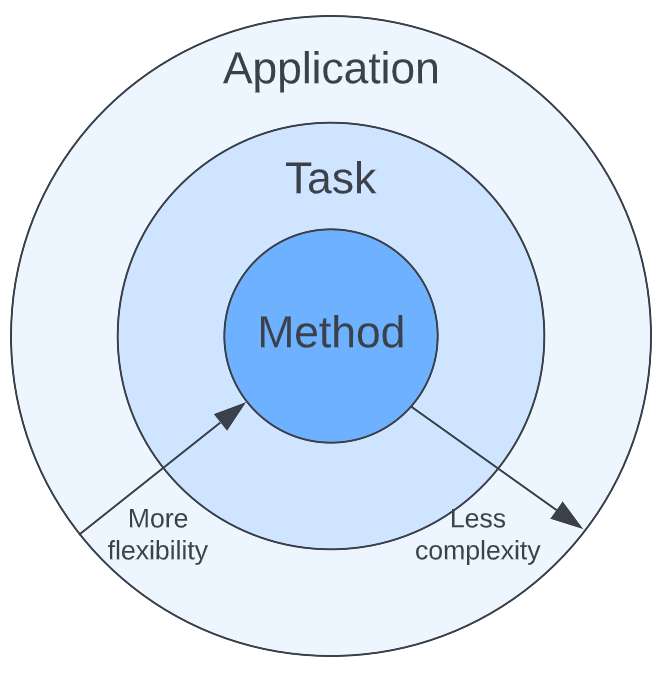
\includegraphics[width=0.4\textwidth]{figures/granularity.png}
	\caption{سه دانه‌بندی مختلف در سامانه تخلیه پردازش}
	\label{fig:granularity}
\end{figure}
به عنوان نمونه در \cite{maui} دانه‌بندی در سطح متد صورت گرفته است، در حالی که در \cite{Liu} دانه‌بندی در سطح وظیفه صورت گرفته است. ما نیز در پژوهش فعلی مسئله تخلیه پردازش را در سطح وظیفه حل کرده‌ایم.
\newpage
\subsection*{تعداد کاربران (\lr{User Count})}
در برخی از مقالات مانند \cite{Liu} مسئله تخلیه پردازش تنها برای یک کاربر در نظر گرفته می‌شود در حالیکه در برخی از پژوهش‌ها مانند \cite{multiuser} از چندین کاربر همزمان نیز پشتیبانی می‌شود. در پژوهش فعلی تعداد کاربران را برای سادگی بیشتر یک در نظر می‌گیریم.

\subsection*{تحرک‌پذیری (\lr{Mobility})}
به انجام پردازش توسط هر گره\LTRfootnote{Node}ای به جز گره ایجاد کننده وظیفه، تخلیه وظیفه گفته می‌شود. طبق این تعریف سه نوع از تحرک‌پذیری را متناظر با نوع گره پردازشی می‌توانیم در نظر بگیریم.
\begin{enumerate}
	\item پردازش در سرور ابری
	\item پردازش در سرور لبه‌ای
	\item پردازش در شبکه‌ای بدون ساختار\LTRfootnote{Ad-hoc} (از دستگاه‌های کاربر)
\end{enumerate}

\subsection*{تعداد سرور}
مشابه با تعداد کاربران، تعداد سرورهای پردازشی در سامانه تخلیه نیز می‌تواند یک یا بیشتر باشد. برای نمونه در \cite{multiuser} مسئله تخلیه پردازش برای چندین سرور بررسی شده است. در پژوهش فعلی ما حالت تک سرور را در نظر می‌گیریم.

\subsection*{معیار بهینه‌سازی}
 معیار بهینه‌سازی به کمیتی اشاره دارد که استراتژی تخلیه پردازش سعی در بهینه‌سازی آن دارد. برخی از معیارهای رایج عبارتند از: تاخیر، انرژی، کیفیت سرویس، و هزینه. برای مثال در \cite{Liu} معیار تاخیر، در \cite{metricenergy} معیار انرژی و در \cite{metriccost} معیار هزینه در نظر گرفته شده است.
\section{بررسی مقالات از نظر روش حل مسئله}
در جدول \ref{table:algorithms} که برگرفته از 
\cite{Shakarami2020}
می‌باشد، یک دسته‌بندی کلی از الگوریتم‌های رایج در حل مسئله تخلیه پردازش مشاهده می‌شود. برای آشنایی بیشتر با این روش ها به
\cite{wang2019}
و \cite{Shakarami2020} رجوع شود. در این مقاله ما از \textbf{الگوریتمی }قطعی\LTRfootnote{Deteministic} بر پایه برنامه‌ریزی خطی برای یافتن \textbf{استراتژی تخلیه} تصادفی\LTRfootnote{Stochastic} استفاده می‌کنیم. 

% Please add the following required packages to your document preamble:
% \usepackage{booktabs}
\begin{table}[H]
	\centering
	\begin{latin}
		\begin{tabular}{@{}ll@{}}
			\toprule
			\textbf{Model} & \textbf{Examples}                                                                                                                                                           \\ \midrule
			Stochastic     & \begin{tabular}[c]{@{}l@{}}Machine learning, \\ Generalized poison distribution, \\ Game theory, \\ Queuing theory, \\ Markov processes, \\ Gaussian processes\end{tabular} \\ \midrule
			Deterministic  & \begin{tabular}[c]{@{}l@{}}Some supervised Machine Learning approaches (e.g., KNN),\\ Linear and non-linear programming, \\ Linear regression equation\end{tabular}        
		\end{tabular}
	\end{latin}
	\caption{تقسیم‌بندی الگوریتم‌های حل مسئله تخلیه پردازش}
	\label{table:algorithms}
\end{table}

\section{پژوهش‌های مرتبط}
در \cite{Liu} مسئله تخلیه وظیفه با تاخیر کمینه با استفاده از روشی مبتنی بر زنجیره مارکوف و برنامه‌ریزی خطی حل شده است. در این پژوهش محیط تک کاربر و تک سرور در نظر گرفته شده است. روش ارائه شده در درازمدت عملکرد بهینه دارد اما چندین کاستی دارد از جمله عدم پشتیبانی از وظایف با نیازمندی‌های پردازشی متفاوت و عدم پشتیبانی از موازی‌سازی. پژوهش فعلی گسترشی بر این مقاله است. \\

در \cite{samanta} یک مکانزیم تخلیه وظیفه با هزینه کمینه برای محیط رایانش لبه‌ای متحرک ارائه شده است. محیط در نظر گرفته شده از نظر ثابت بودن طول بازه‌های زمانی و تفاوت وظایف و همچنین نحوه تعریف مسئله بهینه‌سازی، شبیه به پژوهش ما می‌باشد. اما از نظر معیار و تعداد سرور متفاوت می‌باشد. روش بهینه‌سازی استفاده شده در این مقاله روش «ضرایب لاگرانژ» می‌باشد که عملکرد سریعی دارد اما لزوما جواب بهینه سراسری را پیدا نمی‌کند و فقط جواب‌های بهینه محلی را پیدا می‌کند. \\

در \cite{kwak} و \cite{jiang} مشابه با پژوهش فعلی، ناهمگونی وظایف و تقابل\LTRfootnote{Tradeoff} تاخیر و انرژی در نظر گرفته شده است. با این تفاوت که در این دو مقاله از روش بهینه‌سازی لیاپانوف استفاده شده است. همچنین این دو مقاله مسئله تخلیه وظیفه را در محیط رایانش ابری را در نظر گرفته‌اند و نه رایانش لبه‌ای و همچنین چارچوب نرم‌افزاری ای برای حل مسئله در محیط‌های خاص ارائه نداده اند. \\

در \cite{zhang2013} مسئله تخلیه و زمان‌بندی ارسال و اجرا به صورت همزمان در نظر گرفته شده است و کانال بیسیم به صورت تصادفی مدل شده است و از این ابعاد به پژوهش ما شباهت دارد. معیار بهینه‌سازی در این پژوهش انرژی مصرفی است. روش ارائه شده عملکرد خوبی دارد و به میزان قابل توجی در انرژی مصرفی صرفه‌جویی می‌کند. با این حال مدل در نظر گرفته شده کاستی‌هایی دارد. یک ایراد اصلی فرض وجود تنها یک کاربرد در سیستم است. به عبارت دیگر تاخیر ایجاد شده به واسطه انتظار کاربردها در صف در نظر گرفته نشده است.

\clearpage

\chapter{شرح مسئله}
در این مقاله قصد داریم در یک سامانه رایانش لبه‌ای مطابق با شکل \ref{fig-offloading-system}، استراتژی تخلیه‌ای بیابیم که تاخیر سرویس میانگین $\bar{T}$ را تحت محدودیت توان مصرفی $P_{m a x}$ در درازمدت کمینه کند.
\begin{figure}[H]
	\centering
	\includegraphics*[width=\textwidth]{figures/MEC5.png}
	\caption{ساختار کلی سیستم تخلیه پردازش}
	\label{fig-offloading-system}
\end{figure}
\newpage
همانطور که در شکل \ref{fig-offloading-system} مشاهده می‌شود، در سامانه مد نظر سه مولفه اصلی وجود دارد:
\begin{enumerate}
	\item دستگاه کاربر (\lr{User Equipment})
	\item سرور رایانش لبه‌ای چند-دسترسی (\lr{Multi-access Edge Computing Server})
	\item کانال بیسیم
\end{enumerate}
در فصل جاری نحوه عملکرد هر کدام از این مولفه‌ها در قالب مدل‌های تئوری شرح داده می‌شود.

\section{مدل وظایف}
فرض می‌شود که \(k\) نوع وظیفه مختلف در سیستم رایانش لبه‌ای وجود دارد و به ازای هر نوع وظیفه دقیقا یک صف در سیستم وجود دارد. وظایف نوع \(i\)-اُم برای اجرا به صورت محلی\LTRfootnote{Local} احتیاج به \(L_i\) بازه زمانی پردازش توسط پردازنده دارند و به منظور تخلیه به سرور رایانش لبه‌ای احتیاج به \(M_i\) واحد زمانی ارسال توسط واحد ارسال\LTRfootnote{Transmission Unit} دارند. همچنین فرض می‌شود که وظایف نوع \(i\)-اُم در سرور رایانش لبه‌ای به \(C_i\) بازه زمانی پردازش توسط سرور نیاز دارند. برای سادگی بیشتر در ادامه این مقاله برای اشاره به یک واحد زمانی اجرا توسط پردازنده از عبارت \textbf{«قسمت»}\LTRfootnote{Section} استفاده می‌کنیم که انتزاعی از قسمت‌های کد اجرایی است. و برای اشاره به یک واحد زمانی ارسال توسط واحد ارسال از عبارت\textbf{ «بسته» }استفاده می‌شود.
\newpage
\section{مدل دستگاه کاربر}
\label{sec:ue-model}
دستگاه کاربر مطابق با شکل \ref{fig-offloading-system} شامل دو مولفه پردازنده و واحد ارسال می‌باشد. همچنین همانطور که اشاره شد \(k\) صف مختلف به ازای هر کدام از انواع وظایف در سیستم وجود دارد. ظرفیت هر صف را برابر با مقدار ثابت \(Q\) در نظر می‌گیریم. \\

در هر بازه زمانی، پردازنده یا به اندازه یک قسمت پردازش انجام می‌دهد و یا بیکار\LTRfootnote{Idle} است. اجرای هر قسمت پردازش توسط پردازنده به میزان
\(P_{l o c}\)
وات توان مصرف می‌کند. به طور مشابه واحد ارسال در هر بازه زمانی یا یک بسته را به شبکه ارسال می‌کند یا بیکار است. نکته قابل توجه در مورد واحد ارسال این است که با توجه به شرایط کانال بیسیم، در یک بازه زمانی خاص ممکن است ارسال موفقیت آمیز باشد یا نباشد. فرض می‌شود که ارسال موفقیت آمیز هر بسته به میزان
\(P_{t x}\)
وات توان مصرف می‌کند. توضیحات بیشتر در مورد نحوه کارکرد کانال بی‌سیم در بخش \ref{sec:wireless} آورده شده است. \\

با توجه به توضیحات داده شده می‌توان مدلی برای «حالت دستگاه کاربر»\LTRfootnote{User Equipment State} تعریف کرد. در \cite{Liu} برای مشخص کردن حالت دستگاه در زمان \(t\) از یک سه تایی مانند $\boldsymbol{\tau}[t]=\left(q[t], c_{T}[t], c_{L}[t]\right)$ استفاده شده است، که در آن \(q[t]\) مشخص کننده تعداد وظایف موجود در صف وظایف، \(c_T[t]\) مشخص کننده تعداد بسته ارسال شده از وظیفه تخصیص داده شده به واحد ارسال است، و \(c_L[t]\) مشخص کننده تعداد قسمت اجرا شده از وظیفه تخصیص داده شده به پردازنده است. همچنین حالت \(c_T[t] = 0\) معادل با بیکار بودن واحد ارسال و \(c_L[t] = 0\) معادل با بیکار بودن پردازنده تعریف می‌شود. برای مثال سه تایی \((4, 2, 1)\) به این معنی است که ۴ وظیفه در صف وظایف وجود دارد، واحد پردازش در حال تخلیه وظیفه‌ای است و تا کنون یک بسته از آن وظیفه را ارسال کرده و به عنوان قدم بعدی باید بسته شماره ۲ را ارسال کند. پردازنده نیز در حال اجرای وظیفه‌ای به صورت محلی است و تا کنون یک قسمت از آن وظیفه را اجرا کرده است. \\
\newpage
با این حال مدل فوق در مسئله تخلیه وظیفه با چند نوع وظیفه قابل استفاده نیست و نیاز به تغییر دارد. ما در این مقاله برای تعیین حالت دستگاه کاربر از یک چندتایی\LTRfootnote{Tuple} به طول \(k + 4\) مطابق با رابطه \ref{eg:state} استفاده می‌کنیم. در این رابطه متغیرهای
\(q_1[t], \cdots, q_k[t]\)
تعداد وظایف موجود از هر نوع وظیفه در صف مربوطه را مشخص می‌کنند. متغیرهای \(c_R[t]\) و \(c_L[t]\) مشابه با حالت تک صف تعریف می‌شوند و به ترتیب وضعیت واحد ارسال و پردازنده را مشخص می‌کنند. دو متغیر جدید \(T_R[t]\) و \(T_L[t]\) به ترتیب مشخص کننده نوع وظیفه در حال ارسال توسط واحد ارسال و نوع وظیفه در حال اجرا توسط پردازنده اند.

\begin{equation}
	\label{eg:state}
	\tau[t]=\left(q_{1}[t], q_{2}[t], \ldots, q_{k}[t], c_{R}[t], c_{L}[t], T_{R}[t], T_{L}[t]\right)
\end{equation}
رابطه \ref{eq:state-space} با تعریف شروط مختلف فضای حالت مسئله را توصیف می‌کند. \textbf{(نکته: در رابطه \ref{eq:state-space} و سراسر این مقاله منظور از \(\tau\{X\}\) مقدار متغیر \(X\) در حالت \(\tau\) است.)}

\begin{equation}
	\label{eq:state-space}
	\begin{aligned}
		&\forall \tau \in S, i \in \{1,2, \ldots, k\} \quad 0 \leqslant\tau\left\{q_{i}\right\} \leqslant Q\\
		&\forall \tau \in S \quad  \tau\left\{T_L\right\},  \tau\left\{T_R\right\} \in \{0, 1,2, \ldots, k\}\\
		&\left.\forall \tau \in\left\{\tau^{\prime} \in S \mid \tau^{\prime}\left\{T_{R}\right\}=0\right\} \quad \tau\{C_R\right\}=0\\
		&\forall \tau \in\left\{\tau^{\prime} \in S \mid \tau^{\prime}\left\{T_{R}\right\} \neq 0\right\} \quad 1 \leqslant \tau\left\{C_{R}\right\} \leqslant M_{\tau\{T_{R}\}} \\
		&\left.\forall \tau \in\left\{\tau^{\prime} \in S \mid \tau^{\prime}\left\{T_{L}\right\}=0\right\} \quad \tau\{C_L\right\}=0\\
		&\forall \tau \in\left\{\tau^{\prime} \in S \mid \tau^{\prime}\left\{T_{L}\right\} \neq 0\right\} \quad 1 \leqslant \tau\left\{C_{L}\right\} \leqslant L_{\tau\{T_{L}\}} - 1
	\end{aligned}
\end{equation}

\newpage
\section{مدل زمان}
وضعیت سیستم تخلیه وظیفه در فواصل زمانی\LTRfootnote{Time Slot} با طول ثابت \(\Delta\) میلی ثانیه بررسی می‌شود. برای مثال حالت دستگاه کاربر را در بازه زمانی \(t\)-اُم با \(\tau[t]\) مشخص می‌کنیم، و حالت دستگاه در بازه زمانی \(t + 1\) را با \(\tau[t + 1]\) مشخص می‌کنیم و فاصله بین این دو بازه زمانی \(\Delta\) میلی ثانیه است. \\

بررسی زمان به صورت واحدهای گسسته به منظور ساده‌سازی مسئله و همچنین گسترش پذیری آن به شرایط محیطی مختلف صورت گرفته است. در عمل، یک مقدار قابل استفاده برای \(\Delta\) طول بازه‌های زمانی شبکه دسترسی\LTRfootnote{Access Network} مورد نظر است. برای مثال در شبکه‌های \lr{LTE} طول هر بازه زمانی ۵/۰ میلی‌ثانیه می‌باشد. \cite{LTE}

\section{مدل کانال بیسیم}
\label{sec:wireless}
در این مقاله مشابه با \cite{Liu} کانال بی‌سیم را به صورت تصادفی مدل می‌کنیم\LTRfootnote{Stochastic Channel} یکی از دلایل اصلی برای مدل‌سازی کانال به صورت تصادفی، وجود نویز و ناپایداری در ارتباطات بیسیم است. کانال بی‌سیم را با یک مدل ساده احتمالی دوجمله‌ای  مدل می‌کنیم به این صورت که ارسال هر بسته توسط واحد ارسال با احتمال \(\beta\) موفقیت آمیز خواهد بود و با احتمال \(1 - \beta\) ناموفق خواهد بود. در عمل مقدار \(\beta\) با توجه به رابطه \ref{eq:shannon} (رابطه شنون) محاسبه می‌شود، که در آن \(R\) مشخص کننده سایز هر بسته است،
$r(t)$
مشخص کننده نرخ ارسال در زمان
$t$
،
 \(B\) پهنای باند سیستم، \(\gamma[t]\) مقدار بهره کانال\LTRfootnote{Channel Gain} و \(N_0\) مشخص کننده اندازه نویز کانال است.
\begin{equation}
	\label{eq:shannon}
	\begin{aligned}
		&\beta=P(r(t) \geq R) \\
		&r(t)=B \log _{r}\left(1+\frac{\gamma[t] P_{\mathrm{tx}}}{N_0 B}\right)
	\end{aligned}
\end{equation}
\section{مفهوم کنش}
\label{sec:action}
یک استراتژی تخلیه در هر بازه زمانی مانند \(t\) می‌بایست یک کنش\LTRfootnote{Action} مانند \(A[t]\) را برای اجرا توسط دستگاه کاربر انتخاب کند. اجرای هر کنش می‌تواند حالت دستگاه کاربر را تغییر دهد. برای درک بهتر مفهوم کنش، ابتدا مشابه \cite{Liu} حالتی را در نظر می‌گیریم که تنها یک صف (یک نوع وظیفه) در سیستم وجود داشته باشد. در این حالت می‌توانیم مجموعه کنش‌ها را با چهار عضو مطابق جدول \ref{table:actions} مشخص کنیم.

\begin{table}[H]
	\centering
	\begin{latin}
		\begin{tabular}{@{}lrll@{}}
			\toprule
			\textbf{ID} & \textbf{Transmit} & \textbf{Local Execution} & \textbf{Description} \\ \midrule
			1           & False             & False                    & No operation         \\
			2           & False             & True                     & Add to CPU           \\
			3           & True              & False                    & Add to TU            \\
			4           & True              & True                     & Add to both units    \\ \bottomrule
		\end{tabular}
	\end{latin}
	\caption{لیست کنش‌ها در سیستم با یک صف وظیفه}
	\label{table:actions}
\end{table}
به طور مشابه در شرایطی که بیش از یک نوع وظیفه در سیستم وجود داشته باشد مجموعه کنش‌های ممکن مطابق با جدول \ref{table:actions-multiqueue} بدست می‌آید.
\begin{table}[H]
	\centering
	\begin{latin}
		\begin{tabular}{@{}lrlll@{}}
			\toprule
			\textbf{ID}                     & \textbf{Transmit} & \textbf{Local Execution} & \textbf{Description} & \textbf{Count}                \\ \midrule
			$\{1\}$                           & False             & False                    & No operation         & 1                    \\
			$\{2, ..., k + 1\}$               & False             & True                     & Add to CPU           & $k$                    \\
			$\{k + 2, ..., 2k + 1\}$          & True              & False                    & Add to TU            & $k$                    \\
			$\{2k + 2, ..., 2k + k * k - 1\}$ & True              & True                     & Add to both units    & $k^2$ \\ \bottomrule
		\end{tabular}
	\end{latin}
	\caption{دسته‌بندی کنش‌ها در سیستم با $k$ صف}
	\label{table:actions-multiqueue}
\end{table}
اجرای هر کنش طبعا ممکن است که حالت سیستم را تغییر دهد. به طور مثال اجرای هر کنش نوع \lr{Add To CPU} یک وظیفه را از صف مربوطه بر می‌دارد، بنابراین طول صف مطابق (\(q_i[t + 1] = q_i[t] - 1\) تغییر می‌کند. با اجرای این کنش همچنین وضعیت پردازنده از \(c_L[t] = 0\) یعنی حالت بیکار به \(c_L[t + 1] = 1\) تغییر خواهد کرد زیرا قسمت اول وظیفه مربوطه در بازه زمانی \(t\) انجام خواهد شد. به طور مشابه برای سایر کنش‌ها نیز میتوان توابع انتقال\LTRfootnote{Transition Function} مشخص تعریف کرد که با گرفتن یک حالت ورودی، حالت خروجی را محاسبه نماید. به دلیل پیچیدگی روابط این توابع، از توضیح بیشتر در این بخش صرف نظر شده است. برای مشاهده منطق دقیق این توابع در قالب کد، به پیوست ۱ مراجعه شود.
\section{استراتژی تخلیه}
استراتژی تخلیه در هر بازه زمانی تصمیم می‌گیرد که دستگاه کاربر چه کنشی را اجرا کند. بنابراین استراتژی تخلیه یک تابع مانند $G(\tau)$ می‌باشد که با گرفتن حالت دستگاه کاربر $\tau[t]$ به عنوان ورودی، یک کنش مانند \(a\) را به عنوان خروجی می‌دهد. لازم به ذکر است که در اینجا این تابع را به صورت مفهومی انتزاعی در نظر می‌گیریم و در فصل‌های آتی به طور دقیق به نحوه بدست آوردن تابع بهینه $g(\tau)^{*}$ خواهیم پرداخت.
\newpage
\section{روند فعالیت سیستم تخلیه وظایف}
نحوه عملکرد دستگاه کاربر در هر بازه زمانی مطابق با فرآیند مشخص شده در شکل \ref{fig:ueproc} می‌باشد. در هر باز، دستگاه کاربر ابتدا کنش اجرایی را از یک استراتژی تخلیه دریافت می‌کند. سپس کنش انتخاب شده توسط دستگاه کاربر اجرا خواهد شد که ممکن است منجر به تغییر حالت دستگاه شود. سپس پردازنده و واحد ارسال هر کدام در صورت فعال بودن به اندازه یک بازه زمانی فعالیت خواهند کرد. در انتها وظایف جدید با احتمالات
$\alpha_1, \cdots, \alpha_k$
به صف‌های وظایف اضافه خواهند شد.


\begin{figure}[H]
	\centering
	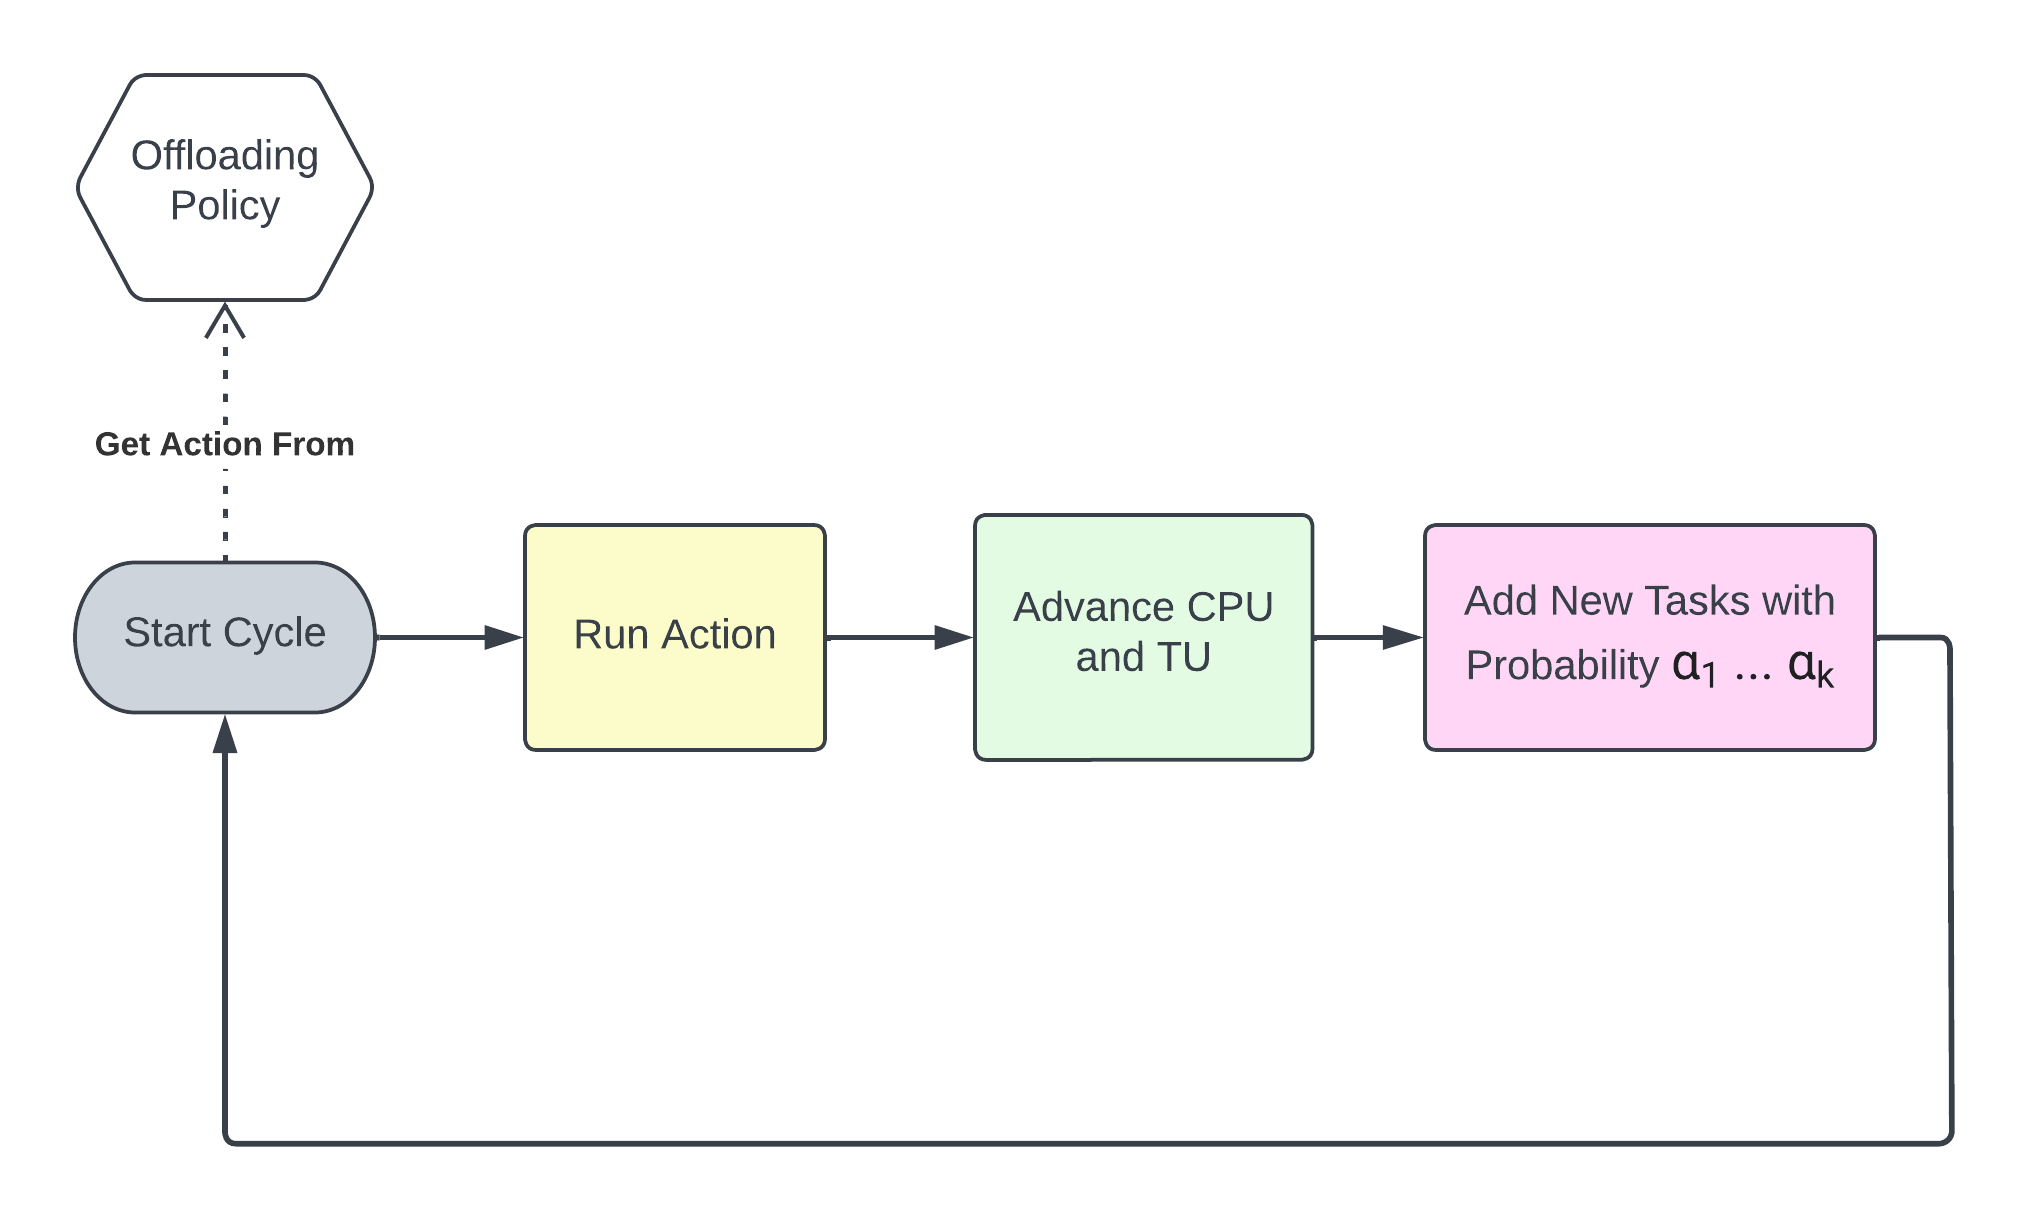
\includegraphics[width=\textwidth]{figures/ueproc.png}
	\caption{روند فعالیت دستگاه کاربر}
	\label{fig:ueproc}
\end{figure}
\chapter{روش پیشنهادی}
در این فصل الگوریتمی ارائه خواهیم داد که با استفاده از آن می‌توان مسئله یافتن استراتژی تخلیه با تاخیر کمینه را که در فصل قبل تشریح شد را حل کرد. استراتژی خروجی توسط الگوریتم از نوع تصادفی می‌باشد و برای بدست آوردن آن از مفاهیمی مانند زنجیره مارکوف و برنامه‌ریزی خطی استفاده خواهد شد.

\section{استراتژی تخلیه تصادفی}
با استفاده از مدل‌های توصیف شده در فصل قبل می‌توانیم یک تعریف ریاضی از «استراتژی تخلیه تصادفی» داشته باشیم. مشابه با مقاله \cite{Liu} استراتژی تخلیه تصادفی را به صورت یک توزیع احتمالی مانند \(g_\tau^a\) بر روی مجموعه \(S \times A\) تعریف می‌کنیم. در اینجا عبارت \(S \times A\) نمایانگر ضرب دکارتی مجموعه تمام حالت‌های سیستم در مجموعه تمام کنش‌های ممکن در سیستم است. یک نکته قابل توجه این است که برخی از دو تایی‌های حاصل از این ضرب دکارتی هیچ گاه در واقعیت امکان‌پذیر نیست. برای مثال در حالتی که صف خالی باشد تنها یک کنش امکان پذیر است و آن هم کنش شماره ۱ (\lr{No Operation}) است. با این حال برای سادگی در توضیح تئوری روش حل مسئله، این دو تایی‌ها را نیز در دامنه تابع توزیع احتمالی استراتژی تخلیه در نظر می‌گیریم تا همواره تعداد اعضای دامنه تابع احتمال برابر با \(|S| \cdot |A|\) باشد. \\

همچنین طبق تعریف توزیع احتمال، رابطه \ref{eq:prob} باید برای هر استراتژی تخلیه تصادفی برقرار باشد.
\begin{equation}
	\label{eq:prob}
	\sum_{\tau \in S} \sum_{a \in A} g_{\tau}^{a}=1
\end{equation}
\section{مدل زنجیره مارکوف دستگاه کاربر}
در این قسمت ابتدا مدل آماری زنجیره مارکوف گسسته-زمان را معرفی می‌کنیم و سپس توضیح می‌دهیم که چگونه می‌توان با استفاده از این مدل معیارهای تاخیر و توان مصرفی میانگین را برای یک سیستم تخلیه وظیفه محاسبه کرد.
\begin{defi}
\label{def:one}
دنباله‌ای از متغیرهای تصادفی $X_{1}, X_{2}, \ldots$ را که احتمال تغییر وضعیت از زمان $t$ به $t + 1$ مستقل از وضعیت‌های قبلی باشد را یک \textbf{زنجیره مارکوف گسسته-زمان} می‌نامند. این گزاره را به بیان متغیرهای تصادفی و تابع احتمال به صورت رابطه زیر نشان می‌دهیم.
\begin{equation*}
	\operatorname{Pr}\left(X_{t+1}=x \mid X_{1}=x_{1}, X_{2}=x_{2}, \ldots, X_{n}=x_{t}\right)=\operatorname{Pr}\left(X_{t+1}=x \mid X_{t}=x_{t}\right)
\end{equation*}
\end{defi}
زنجیره مارکوف گسسته‌-زمان را می‌توان با گراف جهت‌دار نیز نمایش داد. در شکل \ref{fig:gambler} یک زنجیره نمونه مشاهده می‌شود.
\begin{figure}[H]
	\centering
	\begin{latin}
			\begin{tikzpicture}[ - > , shorten >=2pt , line width =0.5 pt , node distance =2 cm]
			\node [circle , draw] (zero) {0};
			\node [circle , draw] (one) [right of=zero] {1};
			\node [circle , draw] (two) [right of=one] {2};
			\node [circle , draw] (three) [right of=two] {3};
			\path (zero) edge [loop left] node {$1$} (zero) ;
			\path (one) edge node [above] {$1 - p$} (zero) ;
			\path (one) edge [bend left] node [above]{$p$} (two) ;
			\path (two) edge node [above]{$p$} (three) ;
			\path (two) edge [bend left] node [below]{$1 - p$} (one) ;
			\path (three) edge [loop right] node {$1$} (three) ;
		\end{tikzpicture}
	\end{latin}
	\caption[یک مارکوف نمونه برای مسئله پاکباختگی]{یک زنجیره مارکوف نمونه برای مسئله پاکباختگی قمارباز\protect\footnotemark}
	\label{fig:gambler}
\end{figure}
\LTRfootnotetext{The Gambler's ruin}
\newpage
\begin{defi}
\label{def:two}
زنجیره مارکوف گسسته زمان $X(t)$ را \textbf{همگن-زمان} می‌گوییم اگر شرط زیر همواره برقرار باشد:
\begin{equation*}
P\left(X_{n+1}=j \mid X_{n}=i\right)=P\left(X_{1}=j \mid X_{0}=i\right)
\end{equation*}
به عبارت دیگر یعنی احتمالات مربوط به انتقال بین حالت‌ها به زمان \(t\) وابسته نیستند. در این حالت احتمال انتقال زنجیره از حالت \(i\) به \(j\) را با عبارت $p_{i j}=P\left(X_{1}=j \mid X_{0}=i\right)$ نمایش می‌دهیم و همچنین ماتریس انتقال را با $P=\left(p_{i j}\right)$ نمایش می‌دهیم. ماتریس انتقال را می‌توان به صورت یک گراف جهت‌دار نیز توصیف کرد به طوری که درایه $p_{i, j}$ در ماتریس معادل یک یال جهت‌دار از راس $i$ به راس $j$ با وزن $p_{i, j}$ است.
\end{defi}
طبق تعاریف \ref{def:one} و \ref{def:two} می‌توان حالت دستگاه کاربر در طی زمان را به صورت یک زنجیره مارکوف گسسته‌زمان در نظر گرفت به طوری که $\tau[t]$ حالت زنجیره در زمان $t$ را مشخص می‌کند. همچنین ماتریس انتقال $\chi$ را اینگونه تعریف می‌کنیم که $\chi_{\tau, \tau^{\prime}}$ احتمال انتقال از حالت $\tau$ به \(\tau^{\prime}\) را مشخص می‌کند. \\

ماتریس انتقال را می‌توان به ازای یک استراتژی تخلیه داده شده و پارامترهای سیستمی مانند \(\alpha_1, \cdots, \alpha_k\) بدست آورد. در شکل \ref{fig:digraph} گراف جهت‌دار معادل زنجیره مارکوف برای یک سیستم با یک صف وظیفه و \(Q = 2\) و تعداد ۲ قسمت به ازای هر وظیفه و تعداد ۱ بسته به ازای هر وظیفه رسم شده است.\footnote{کد استفاده شده برای رسم این گراف در آدرس \lr{https://github.com/dalisyron/OffloadingVisualizer} موجود می‌باشد}
\begin{figure}[H]
\centering
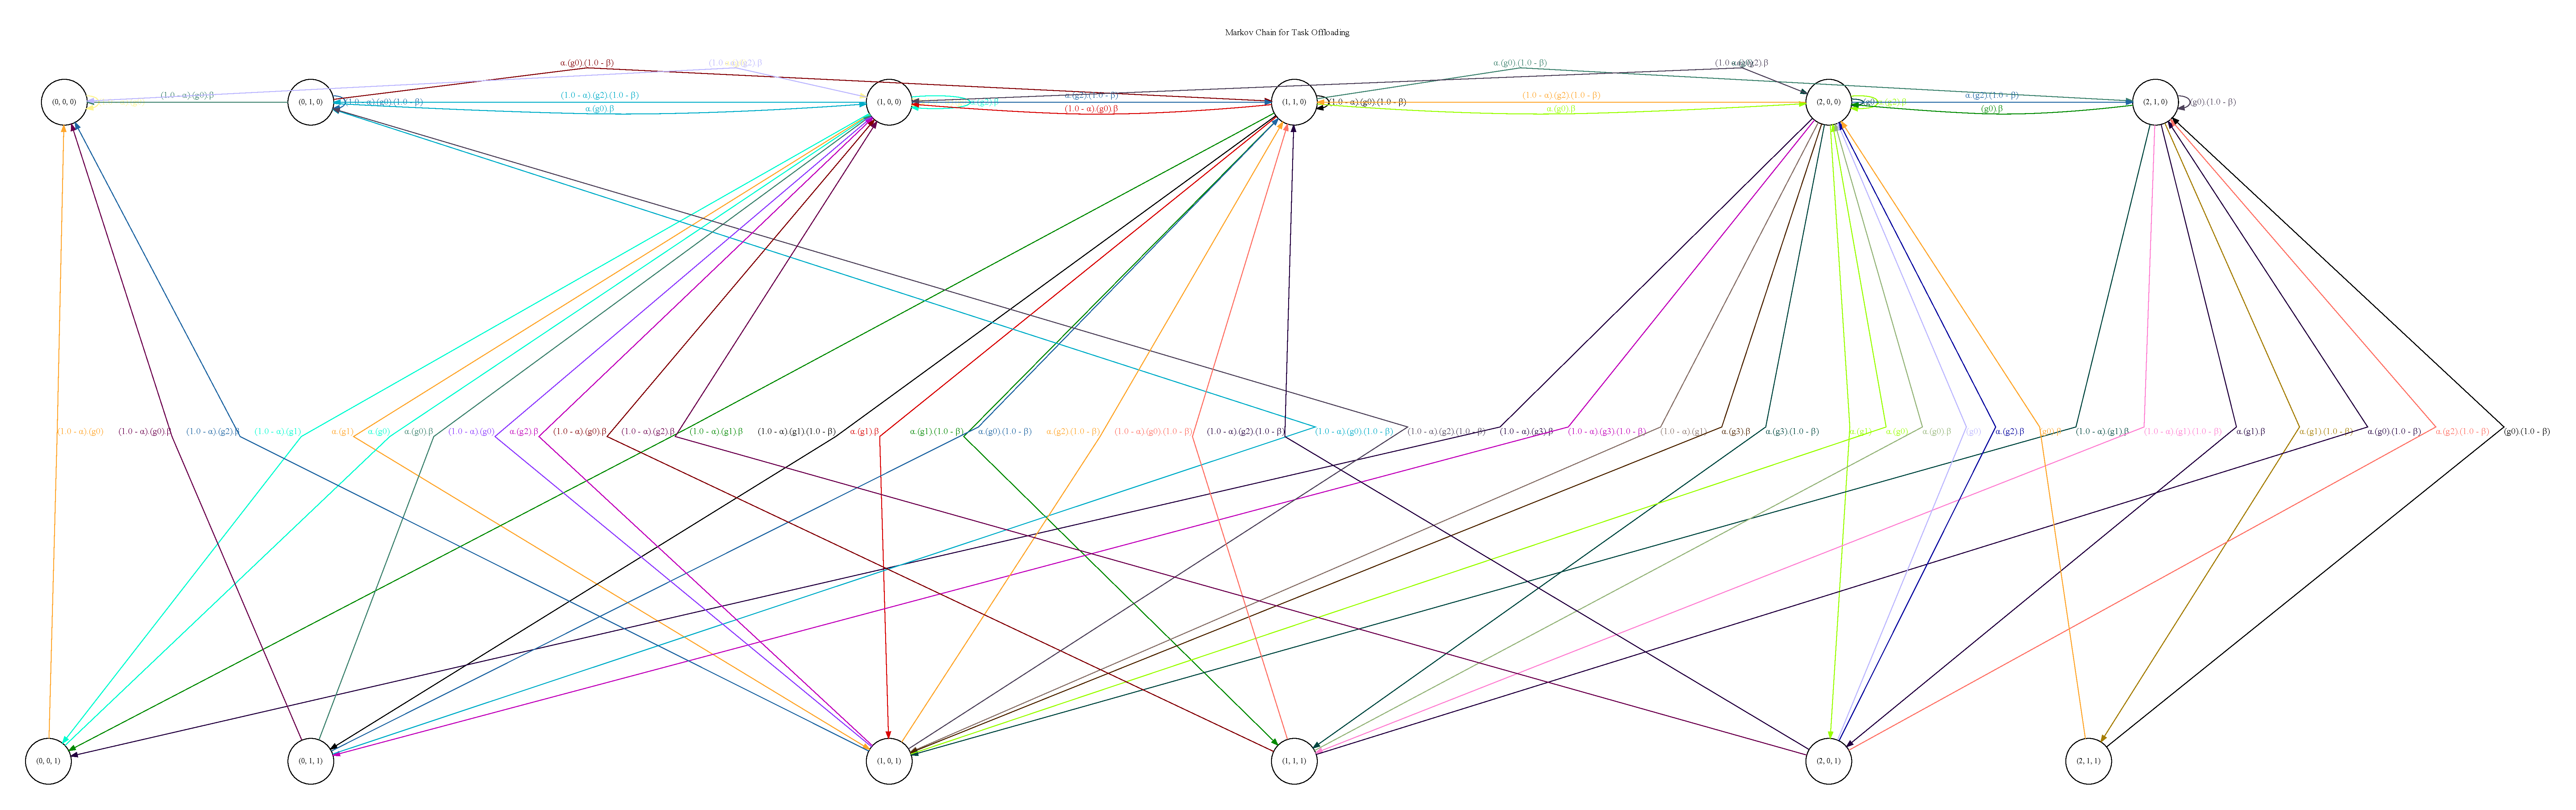
\includegraphics[width=\textwidth]{figures/graph.pdf}
\caption[زنجیره مارکوف سیستم تخلیه در قالب گراف جهت دار]{
زنجیره مارکوف سیستم تخلیه در قالب گراف جهت دار (برای مشاهده جزئیات زوم کنید)
}
\label{fig:digraph}
\end{figure}
به منظور محاسبه معیارهایی مانند توان مصرفی میانگین و تاخیر سرویس میانگین لازم است که بتوانیم درباره وضعیت سیستم تخلیه وظیفه در طولانی‌مدت استنتاج کنیم. در همین راستا مفهوم توزیع پایدار را تعریف می‌کنیم.
\begin{defi}
توزیع احتمالی مانند $p_i$ را یک \textbf{توزیع پایدار} برای زنجیره مارکوف با ماتریس انتقال \(P\) می‌گوییم هر گاه شرط زیر در آن برقرار باشد:
\begin{equation*}
	\pi=\pi P \quad \Longleftrightarrow \quad \pi_{j}=\sum_{i} \pi_{i} P_{i j} \quad \forall j .
\end{equation*}
\end{defi}
یک سوالی که ممکن است بوجود بیاید این است که آیا هر زنجیره مارکوف گسسته‌زمان توزیع پایدار دارد؟ برای پاسخ به این سوال لازم است دو مفهوم زنجیره مارکوف تقلیل‌ناپذیر و غیرمتناوب را تعریف کنیم.
\begin{defi}
اگر رسیدن از هر نقطه به نقطه دیگر از فضای حالت با احتمال مثبت در زنجیره مارکوف میسر باشد، زنجیره را \textbf{تقلیل‌ناپذیر} گویند. به بیان ریاضی می‌توان تقلیل‌ناپذیر بودن زنجیره مارکوف را به صورت زیر نشان داد.
\begin{equation*}
	\operatorname{Pr}\left(X_{n_{i j}}=j \mid X_{0}=i\right)=p_{i j}^{\left(n_{i j}\right)}>0
\end{equation*}
\end{defi}

\begin{defi}
تناوب $d(i)$ برای حالت $i$ به صورت $d(i)=\operatorname{gcd}\left\{n: P_{i i}^{n}>0\right\}$ تعریف می‌شود، که به معنی بزرگ‌ترین مقسوم علیه مشترک تعداد مراحل ممکن است به صورتی که از $i$ شروع کرده و به $i$ برگردیم. یک زنجیره مارکوف تقلیل‌ناپذیر را متناوب با تناوب $d$ می‌گوییم اگر تمامی حالت‌ها تناوبی برابر با $d > 1$ را داشته باشند. یک زنجیره مارکوف تقلیل ناپذیر را \textbf{غیرمتناوب} می‌گوییم اگر تمامی حالت‌ها تناوب برابر با ۱ داشته باشند.
\end{defi}
\begin{thm}
\label{thm:converge}
\textbf{(همگرایی)}
هر زنجیره مارکوف تقلیل‌ناپذیر و غیر متناوب دارای یک توزیع پایدار منحصر به فرد مانند $\pi$ می‌باشد.
\end{thm}
حال با استفاده از قضیه \ref{thm:converge} ثابت می‌کنیم که زنجیره مارکوف سیستم تخلیه وظیفه دارای توزیع پایدار منحصر به فرد است. برای سادگی فرض می‌کنیم که سامانه یک صف دارد و سپس نحوه بسط نتیجه به چندین صف را توضیح می‌دهیم.

\begin{thm}
\label{thm:irreducible}
زنجیره مارکوف مربوط به سیستم تخلیه تک صف تقلیل ناپذیر است. \\
\textbf{اثبات:} \\
قسمت الف) با توجه به تعریف سیستم تخلیه می‌دانیم که از هر حالت غیر شروع مانند \( (0, 0, 0) \neq (x, y, z)\) می‌توان به حالت شروع رفت. به این منظور کافی است که تمام وظایف داخل صف به نحوی (اجرا یا ارسال) به اتمام برسند و وظیفه جدیدی نیز در این حین وارد سیستم نشود. \\

قسمت ب) همچنین می‌توان ثابت کرد که از حالت شروع \((0, 0, 0)\) می‌توان به هر حالت دیگر \((x, y, z)\) رفت. به این منظور دنباله رخدادهای زیر را در نظر بگیرید:
\begin{enumerate}
	\item ورود \(x\) وظیفه جدید
	\item انتقال یک وظیفه به واحد ارسال و ورود یک وظیفه جدید، هر دو در صورتی که \(y > 0\)
	\item پیشرفت واحد ارسال به مدت \(y\) سیکل و عدم ورود وظیفه جدید در این حین
	\item انتقال یک وظیفه به پردازنده و ورود یک وظیفه جدید، هر دو در صورتی که \(z > 0\)
	\item پیشرفت واحد ارسال به مدت \(z\) سیکل و عدم ورود وظیفه جدید در این حین
\end{enumerate}
با توجه به نتایج بخش الف و ب می‌توان نتیجه گرفت که از گشتی با احتمال مثبت از هر حالت به حالت دیگر وجود دارد بنابراین طبق تعریف زنجیره تقلیل‌ناپذیر است.
\end{thm}
\begin{thm}
\label{thm:aperiodic}
زنجیره مارکوف مربوط به سیستم تخلیه تک صف غیر متناوب است. \\
\textbf{اثبات:} \\
به منظور اثبات این قضیه فقط کافی است که به این نکته توجه کنیم که حالت \((0, 0, 0)\) دارای تناوب یک می‌باشد زیرا با احتمالی مثبت (متناظر با رخداد عدم ورود وظیفه و کنش \lr{No Operation}) می‌توان در همان حالت ماند. با توجه به همین نکته و تقلیل‌ناپذیر بودن زنجیره میتوانیم نتیجه بگیریم که سایر حالت‌ها نیز باید تناوب یک داشته باشند. بنابراین زنجیره غیرمتناوب است.
\end{thm}
با توجه به قضایای \ref{thm:irreducible} و \ref{thm:aperiodic} و قضیه همگرایی می‌توان نتیجه گرفت که زنجیره مارکوف سیستم تخلیه تک صف دارای توزیع پایدار منحصر به فرد می‌ مطابق با رابطه \ref{eq:steady} می‌باشد. برای بسط این اثبات به حالت چند صف اثبات غیرمتناوب بودن یکسان خواهد بود و در اثبات تقلیل‌ناپذیر بودن، رخداد اول به ورود \(x_1, \cdots, x_k\) وظیفه از انواع مختلف تغییر پیدا می‌کند.
\begin{equation}
	\label{eq:steady}
	\left\{\begin{array}{l}
		\sum_{\boldsymbol{\tau}^{\prime} \in \mathcal{S}} \chi_{\boldsymbol{\tau}^{\prime}, \boldsymbol{\tau}} \pi_{\boldsymbol{\tau}^{\prime}}=\pi_{\boldsymbol{\tau}}, \forall \boldsymbol{\tau} \in \mathcal{S} \\
		\sum_{\boldsymbol{\tau} \in \mathcal{S}} \pi_{\boldsymbol{\tau}}=1
	\end{array}\right.
\end{equation}
\section{محاسبه تاخیر میانگین}
تاخیر هر وظیفه شامل تاخیر انتظار در صف وظایف و تاخیر پردازش می‌باشد. به منظور بدست آوردن تاخیر میانگین سیستم ابتدا $\theta_i$ را به عنوان کسری از وظایف سیستم در طولانی مدت که از نوع $i$ هستند تعریف می‌کنیم. اگر طول صف‌ها به مقدار کافی بزرگ باشد و همچنین استراتژی تخلیه‌ای داشته باشیم که منجر به پر شدن صف و اتلاف وظیفه\LTRfootnote{Task Loss} نشود مقدار $\theta_i$ طبق رابطه \ref{eq:theta} بدست می‌آید.
\begin{equation}
\label{eq:theta}
\theta_i = \frac{\alpha_i}{\sum_{j=1}^{k} \alpha_{j}}
\end{equation}
\newpage
پارامتر \(t_q^i\) را برابر با مقدار میانگین تاخیر انتظار در صف مربوط به وظایف نوع $i$ تعریف می‌کنیم. طبق قانون \lr{Little} می‌توان مقدار این تاخیر را بر اساس رابطه \ref{eq:queuing-delay} بدست آورد. همانطور که پیش‌تر ذکر شد برای برقراری این رابطه لازم است که اتلاف وظیفه در صف هیچ‌گاه رخ ندهد. به عبارت دیگر با فرض اینکه استراتژی تخلیه‌ی ارائه شده «کارامد» باشد این رابطه برقرار است. در پیاده‌سازی عملی، محدودیت «کارآمد» بودن یک استراتژی بدین گونه تعریف شده است که احتمال پر بودن صف حداکثر مقداری ناچیز  باشد.

\begin{equation}
	\label{eq:queuing-delay}
	t_{q}^i=\frac{\theta_i}{\alpha_i} \sum_{j=0}^{Q} i \cdot \operatorname{Pr}\{q_i[t]=i\}=\frac{1}{\alpha} \sum_{\tau \in S} \tau\{q_i\} \cdot \pi_{\tau}
\end{equation}
همچنین $t_{tx}^i$ را به عنوان تاخیر ارسال میانگین یک وظیفه از نوع \(i\) توسط واحد ارسال تعریف می‌کنیم که مقدار آن بر اساس امید ریاضی موفقیت در فرآیند برنولی مطابق با رابطه \ref{eq:bernouli} بدست می‌آید.
\begin{equation}
	\label{eq:bernouli}
	t_{t x}^i=M_i \sum_{j=1}^{\infty} j(1-\beta)^{(j-1)} \beta
\end{equation}
به یاد داریم که مقدار تاخیر در صورت پردازش محلی برای وظایف نوع $i$ برابر $L_i$ می‌باشد. تاخیر اجرا در صورت تخلیه وظیفه به صورت مجموع زمان ارسال وظیفه
$t_{tx}^i$
زمان اجرا در سرور لبه‌ای
$C_i$
و تاخیر دریافت نتیجه از سرور
$t_{rx}^i$
محاسبه می‌شود.
\begin{equation}
	t_{c}^i=t_{t x}^i+C_i+t_{rx}
\end{equation}
در نتیجه می‌توان تاخیر اجرای میانگین وظایف نوع $i$ را نیز مطابق رابطه \ref{eq:proc-delay} بیان کرد.
\begin{equation}
	\label{eq:proc-delay}
	t_{p}^i=\eta_i L_i+(1-\eta_i) t_{c}^i
\end{equation}
که در آن
$\eta_i$
بیانگر کسری از وظایف نوع $i$ می‌باشد که در طولانی‌مدت به صورت محلی اجرا می‌شوند و مطابق با رابطه \ref{eq:eta} بدست می‌آيد.
\begin{equation}
	\label{eq:eta}
	\eta_i=\frac{\sum_{\boldsymbol{\tau, a} \in \mathcal{S}_{1}^i\cup\mathcal{S}_{3}^i\cup\mathcal{S}_{5}^i} \pi_{\boldsymbol{\tau}} g_{\boldsymbol{\tau}}^{a} }{\sum_{\boldsymbol{\tau, a} \in \mathcal{S}_{1}^i\cup\mathcal{S}_{2}^i\cup\mathcal{S}_{3}^i\cup\mathcal{S}_{4}^i} \pi_{\boldsymbol{\tau}} g_{\boldsymbol{\tau}}^{a} + 2 \sum_{\boldsymbol{\tau, a} \in S_5^i} \pi_{\boldsymbol{\tau}} g_{\boldsymbol{\tau}}^{a}}
\end{equation}
که در آن
$S_1^i, \cdots, S_5^i$
به صورت زیر تعریف می‌شوند:
\begin{equation}
	\begin{aligned}
		& S_1^i = \{\boldsymbol{\tau, a} \in \mathcal{S} \times A | type(a) = AddToCPU \land locType(a) = i\} \\
		& S_2^i = \{\boldsymbol{\tau, a} \in \mathcal{S} \times A | type(a) = AddToTU \land offloadType(a) = i\} \\ 
		& S_3^i = \{\boldsymbol{\tau, a} \in \mathcal{S} \times A | type(a) = AddToBoth \land locType(a) = i \land offloadType(a) \neq i\} \\
		& S_4^i = \{\boldsymbol{\tau, a} \in \mathcal{S} \times A | type(a) = AddToBoth \land locType(a) \neq i \land offloadType(a) = i\} \\
		& S_5^i = \{\boldsymbol{\tau, a} \in \mathcal{S} \times A | type(a) = AddToBoth \land locType(a) = i \land offloadType(a) = i\}
	\end{aligned}
\end{equation}
در رابطه فوق تابع $type(a)$ نوع کنش را مشخص می‌کند و یکی از چهار نوع بیان شده در بخش \ref{sec:action} می‌باشد. توابع
$locType(a)$
و
$offloadType(a)$
نیز نوع وظیفه مربوط به کنش $a$ را مشخص می‌کنند. \\

با استفاده از روابط بالا همچنین می‌توانیم میانگین تاخیر سرویس هر وظیفه در سیستم را طبق رابطه \ref{eq:total-delay} محاسبه کنیم. رابطه بدست آمده برای $\bar{T}$ همچنین مشخص کننده تابع هدف در مسئله پیدا کردن استراتژی تخلیه بهینه می‌باشد.
\begin{equation}
	\label{eq:total-delay}
	\bar{T}=\sum_{i=1}^{k} \theta_{i}\left(t_{q}^{i}+t_{p}^{i}\right)
\end{equation}
\newpage
\section{توان مصرفی میانگین}
اگر پارامتر
$\mu_\tau^{loc}$
و 
$\mu_\tau^{tx}$
را که به ترتیب به عنوان احتمال فعالیت پردازنده در حالت
$\tau$
و احتمال فعالیت واحد ارسال در حالت
$\tau$
تعریف کنیم، آنگاه توان مصرفی میانگین طبق رابطه زیر بدست می‌آید:
\begin{equation}
	\bar{P}=\sum_{\boldsymbol{\tau} \in \mathcal{S}} \pi_{\boldsymbol{\tau}}\left(\mu_{\boldsymbol{\tau}}^{l o c} P_{l o c}+\mu_{\boldsymbol{\tau}}^{t x} P_{t x}\right)
\end{equation}

\section{استراتژی تخلیه وظیفه بهینه}
\label{sec:strat}
با توجه به توابع بدست آمده برای تاخیر و توان مصرفی میانگین در بخش‌های پیشین، حال می‌توانیم مسئله پیدا کردن استراتژی تخلیه بهینه را به صورت یک مسئله بهینه سازی مانند
$\mathcal{P}_{1}$
بیان کنیم:
\begin{equation}
		\begin{aligned}
			\mathcal{P}_{1}: \min _{\left\{g_{\tau}^{a}\right\}}\; & \bar{T} = (\sum_{i=1}^{k} \frac{1}{\alpha_i} \sum_{\tau \in S} \tau\{q_i\} \cdot \pi_{\tau}) + T_p^0 \\
			\text { \lr{s.t.} } &\left\{\begin{array}{l}
				\bar{P} \leq \bar{P}_{\max } \\
				\sum_{\boldsymbol{\tau}^{\prime} \in \mathcal{S}} \chi_{\boldsymbol{\tau}^{\prime}, \boldsymbol{\tau}} \pi_{\boldsymbol{\tau}^{\prime}}=\pi_{\boldsymbol{\tau}}, \boldsymbol{\tau} \in \mathcal{S}, \\
				\sum_{\boldsymbol{\tau} \in S} \pi_{\boldsymbol{\tau}}=1, \\
				\sum_{\alpha \in A} g_{\tau}^{\alpha}=1, \forall \tau \in S\\
				g_{\tau}^{a} \geq 0, \forall \tau \in S,\;a \in A
			\end{array}\right.
		\end{aligned}
\end{equation}
که در آن
$T_p^0$
برابر با تاخیر اجرای میانگین است که به ازای مقادیر داده شده از
$\eta_0, \cdots, \eta_k$
مقداری ثابت دارد و از رابطه زیر بدست می‌آید:
\begin{equation}
	T_p^0 = \sum_{i=1}^{k} (\eta_i L_i+(1-\eta_i) t_{c}^i)
\end{equation}
\clearpage
مسئله
$\mathcal{P}_{1}$
به دلیل وجود پارامتر $\eta_i$ در تابع هدف یک مسئله خطی نیست. با این حال می‌توانیم با استفاده از تغییری کوچک مسئله را به مجموعه‌ای از مسائل برنامه‌ریزی خطی تبدیل کنیم. به این منظور مشابه با \cite{Liu} ابتدا از تعریف «معیار احاطه\LTRfootnote{Occupation Measure}» در زنجیره مارکوف استفاده می کنیم. به این منظور مجموعه متغیرهای جایگزین $\left\{x_{\tau}^{a}\right\}$ را طبق رابطه $x_{\tau}^{a}=\pi_{\tau} g_{\tau}^{a}$ تعریف می‌کنیم. به عبارتی $x_{\tau}^{a}$ برابر با احتمال حضور در حالت $\tau$ و انتخاب کنش
$a$
می‌باشد. همچنین طبق تعریف می‌دانیم که
$\sum_{a \in A} g_{\tau}^{a}=1$
بنابراین خواهیم داشت
$\pi_{\boldsymbol{\tau}}=\sum_{a \in A} x_{\boldsymbol{\tau}}^{a}$
\\\\
حال با جایگذاری $\left\{x_{\tau}^{a}\right\}$ به جای $\{\pi_\tau\}$ در
$\mathcal{P}_{1}$
خواهیم داشت:
\begin{equation}
	\label{eq:p2}
	\begin{aligned}
		\mathcal{P}_{2}: \min _{\boldsymbol{x}, \eta}\; & \bar{T}=(\sum_{i=1}^{k} \frac{1}{\alpha_i} \sum_{\tau \in \mathcal{S}} \sum_{a \in A} \tau\{q_i\} \cdot x_{\tau}^{a})+ T_p^0 \\
		\text { \lr{s.t.} } &\left\{\begin{array}{l}
			\nu_{l o c}(\boldsymbol{x}) P_{l o c}+\beta \nu_{t x}(\boldsymbol{x}) P_{t x} \leq \bar{P}_{\max } \\
			\Gamma(\boldsymbol{x}, \eta_i)=, \forall i \in \{1, \cdots, k\}\\
			F_{\tau}(\boldsymbol{x})=0, \forall \tau=(i, m, n) \in \mathcal{S} \\
			\sum_{\tau \in \mathcal{S}} \sum_{a \in A}=1 \\
			\eta_i \in [0, 1], \forall i \in \{1, \cdots, k\} \\
			x_{\tau}^{a} \geq 0, \forall \tau \in S, a \in A
		\end{array}\right.
	\end{aligned}
\end{equation}
که در آن
$\nu_{l o c}$
و
$\nu_{t x}$
به ترتیب احتمال فعالیت پردازنده و واحد ارسال را در یک واحد زمانی دلخواه مشخص می‌کنند و به ازای یک استراتژی داده شده قابل محاسبه اند. \footnote{برای مشاهده روش محاسبه این دو پارامتر در قالب کد به پیوست ۲ مراجعه شود.} تابع
$\Gamma(\boldsymbol{x}, \eta_i)$
بر اساس رابطه \ref{eq:eta} می‌باشد و به صورت زیر محاسبه می‌شود:
\begin{equation}
	\Gamma(x, \eta) = \eta  \sum_{\boldsymbol{\tau, a} \in \mathcal{S}_{1}^i\cup\mathcal{S}_{2}^i\cup\mathcal{S}_{3}^i\cup\mathcal{S}_{4}^i} x_{\tau}^a + 2 \eta \sum_{\boldsymbol{\tau, a} \in S_5^i} x_{\tau}^a
	- \eta \sum_{\boldsymbol{\tau, a} \in \mathcal{S}_{1}^i\cup\mathcal{S}_{3}^i\cup\mathcal{S}_{5}^i} x_{\tau}^a
\end{equation}
و تابع 
$F_{\tau}(\boldsymbol{x})$
به صورت زیر تعریف می‌شود:
\begin{equation}
	F_{\tau}(\boldsymbol{x})=\sum_{\tau^{\prime} \in \mathcal{S}} \sum_{a \in A} \tilde{\chi}_{\tau^{\prime}, \tau, a} x_{\tau^{\prime}}^{a}-\sum_{a \in A} x_{\tau}^{a}
\end{equation}
در رابطه فوق منظور از
$ \tilde{\chi}_{\tau^{\prime}, \tau, a}$
احتمال شرطی این است که به شرط اینکه در حالت
$\tau^{\prime}$
باشیم و کنش
$a$
انتخاب شده باشد، آنگاه به حالت
$\tau^{\prime}$
برویم. \\

در صورتی که مقادیر
$\eta_0, \cdots, \eta_k$
معلوم باشد آنگاه مسئله
$\mathcal{P}_2$
تبدیل به یک مسئله برنامه‌ریزی خطی می‌شود. با یافتن مقادیر جواب بهینه
$\left\{x_{\tau}^{a}\right\}$ 
می‌توان استراتژی بهینه را طبق رابطه زیر بدست آورد:
\begin{equation}
	g_{\tau}^{a *}=\frac{x_{\tau}^{a *}}{\sum_{a \in A} x_{\tau}^{a *}}, \forall \tau \in \mathcal{S}, a \in A
\end{equation}
بنابراین جهت یافتن استراتژی بهینه برای یک سیستم تخلیه وظیفه کافی است که مسئله برنامه‌ریزی خطی حاصل از
$\mathcal{P}_2$
را به ازای مقادیر مختلف 
$\eta_0, \cdots, \eta_k$
حل کرده تا استراتژی بهینه بدست بیاید. مراحل این فرآیند جستجو در الگوریتم ۱ به صورت خلاصه آمده است.

\begin{latin}
	\begin{algorithm}
		\rl{\caption{الگوریتم جستجوی استراتژی تخلیه وظیفه بهینه}\label{alg:cap}}
		\begin{algorithmic}[1]
			\Require $precision \geq 2$
			\State $etaSettings \gets splitRange([0, 1], precision)^k$
			\State $optimalPolicy = null$
		    \ForEach {$s \in etaSettings$}
				\State $(\eta_0, \cdots, \eta_k) \gets s$
				\State $solution \gets solveLP(\eta_0, \cdots, \eta_k)$
				\If{$optimalPolicy = null\;\mathbf{or}\;solution.delay < optimalPolicy.delay$}
					\State $optimalPolicy \gets solution.policy$
				\EndIf
			\EndFor \\
			\Return $optimalPolicy$
		\end{algorithmic}
	\end{algorithm}
\end{latin}

\section{دو بهینه‌سازی برای الگوریتم جستجوی استراتژی}
\label{sec:optim}
در این بخش دو بهینه‌سازی مختلف را به منظور بهبود عملکرد الگوریتم \ref{alg:cap} معرفی می‌کنیم. این دو بهینه‌سازی در فریم‌ورک \lr{Kompute} که در بخش پیش رو ارائه خواهد شد پیاده‌سازی شده اند.

\subsection{کاهش تعداد متغیرها}
\label{sub:reducevariable}
در مسئله بهینه‌سازی 
$\mathcal{P}_2$
تعداد 
$|S| \cdot |A|$
متغیر وجود دارد. این مقدار برای تعداد صف‌های کم (برای مثال $k \leq 4$) قابل اجرا می‌باشد اما با افزایش تعداد صف‌ها اجرای الگوریتم را بسیار زمان‌بر و یا غیرممکن می‌کند. یک بهینه‌سازی خیلی ساده ولی کارآمد که در \cite{Liu} به آن اشاره‌ای نشده است این است که می‌توان تمام متغیرهای مانند
$x_{\tau}^{a}$
که کنش
$a$
جزو کنش‌های ممکن در
$\tau$
نباشد را حذف کرد زیرا مقدار آنها در جواب مسئله همواره برابر صفر می‌باشد.

\subsection{موازی‌سازی}
الگوریتم \ref{alg:cap} به گونه‌ای تعریف شده است که امکان موازی‌سازی و مقیاس‌پذیری\LTRfootnote{Scaling} آن به صورت خطی وجود دارد. به عبارت دیگر می‌توان مسئله برنامه‌ریزی خطی متناظر با هر مقداردهی از
$\eta_0, \cdots, \eta_k$
را به یک هسته/گره پردازشی خاص اختصاص داد. در شبیه‌سازی سناریو وظایف سبک و سنگین (رجوع شود به \ref{sub:heavylight}) مشاهده شد که الگوریتم موازی‌سازی شده هنگام اجرا بر روی سروری با ۲۴ هسته و تقسیم‌بندی به ۲۴ رشته\LTRfootnote{Thread} عملکردی معادل ۲۰ برابر سریع‌تر از حالت تک‌رشته\LTRfootnote{Single-thread} داشت.
\chapter{آزمایش و نتایج}
\section{ساختار نرم‌افزاری \lr{Kompute}}
به منظور تست الگوریتمی که در بخش پیشین ارائه گردید، یک ساختار نرم‌افزاری (فریم‌ورک) با نام \lr{Kompute} در زبان \lr{Kotlin} تعبیه شده است. با استفاده از این فریم‌ورک می‌توان الگوریتم جستجوی استراتژی تخلیه بهینه را به ازای پارامترهای محیطی مختلف پیدا کرد و با کمک شبیه‌سازی نتایج آن را با سایر استراتژی‌ها مقایسه کرد. این فریم‌ورک طبق یافته‌های ما اولین پیاده‌سازی متن‌باز در زمینه استراتژی‌های تخلیه وظیفه ناهمگون است. \\
معماری کلی این فریم‌ورک در قالب یک کلاس دیاگرام ساده شده در صفحه بعد آورده شده است.
\newpage
\begin{figure}[H]
	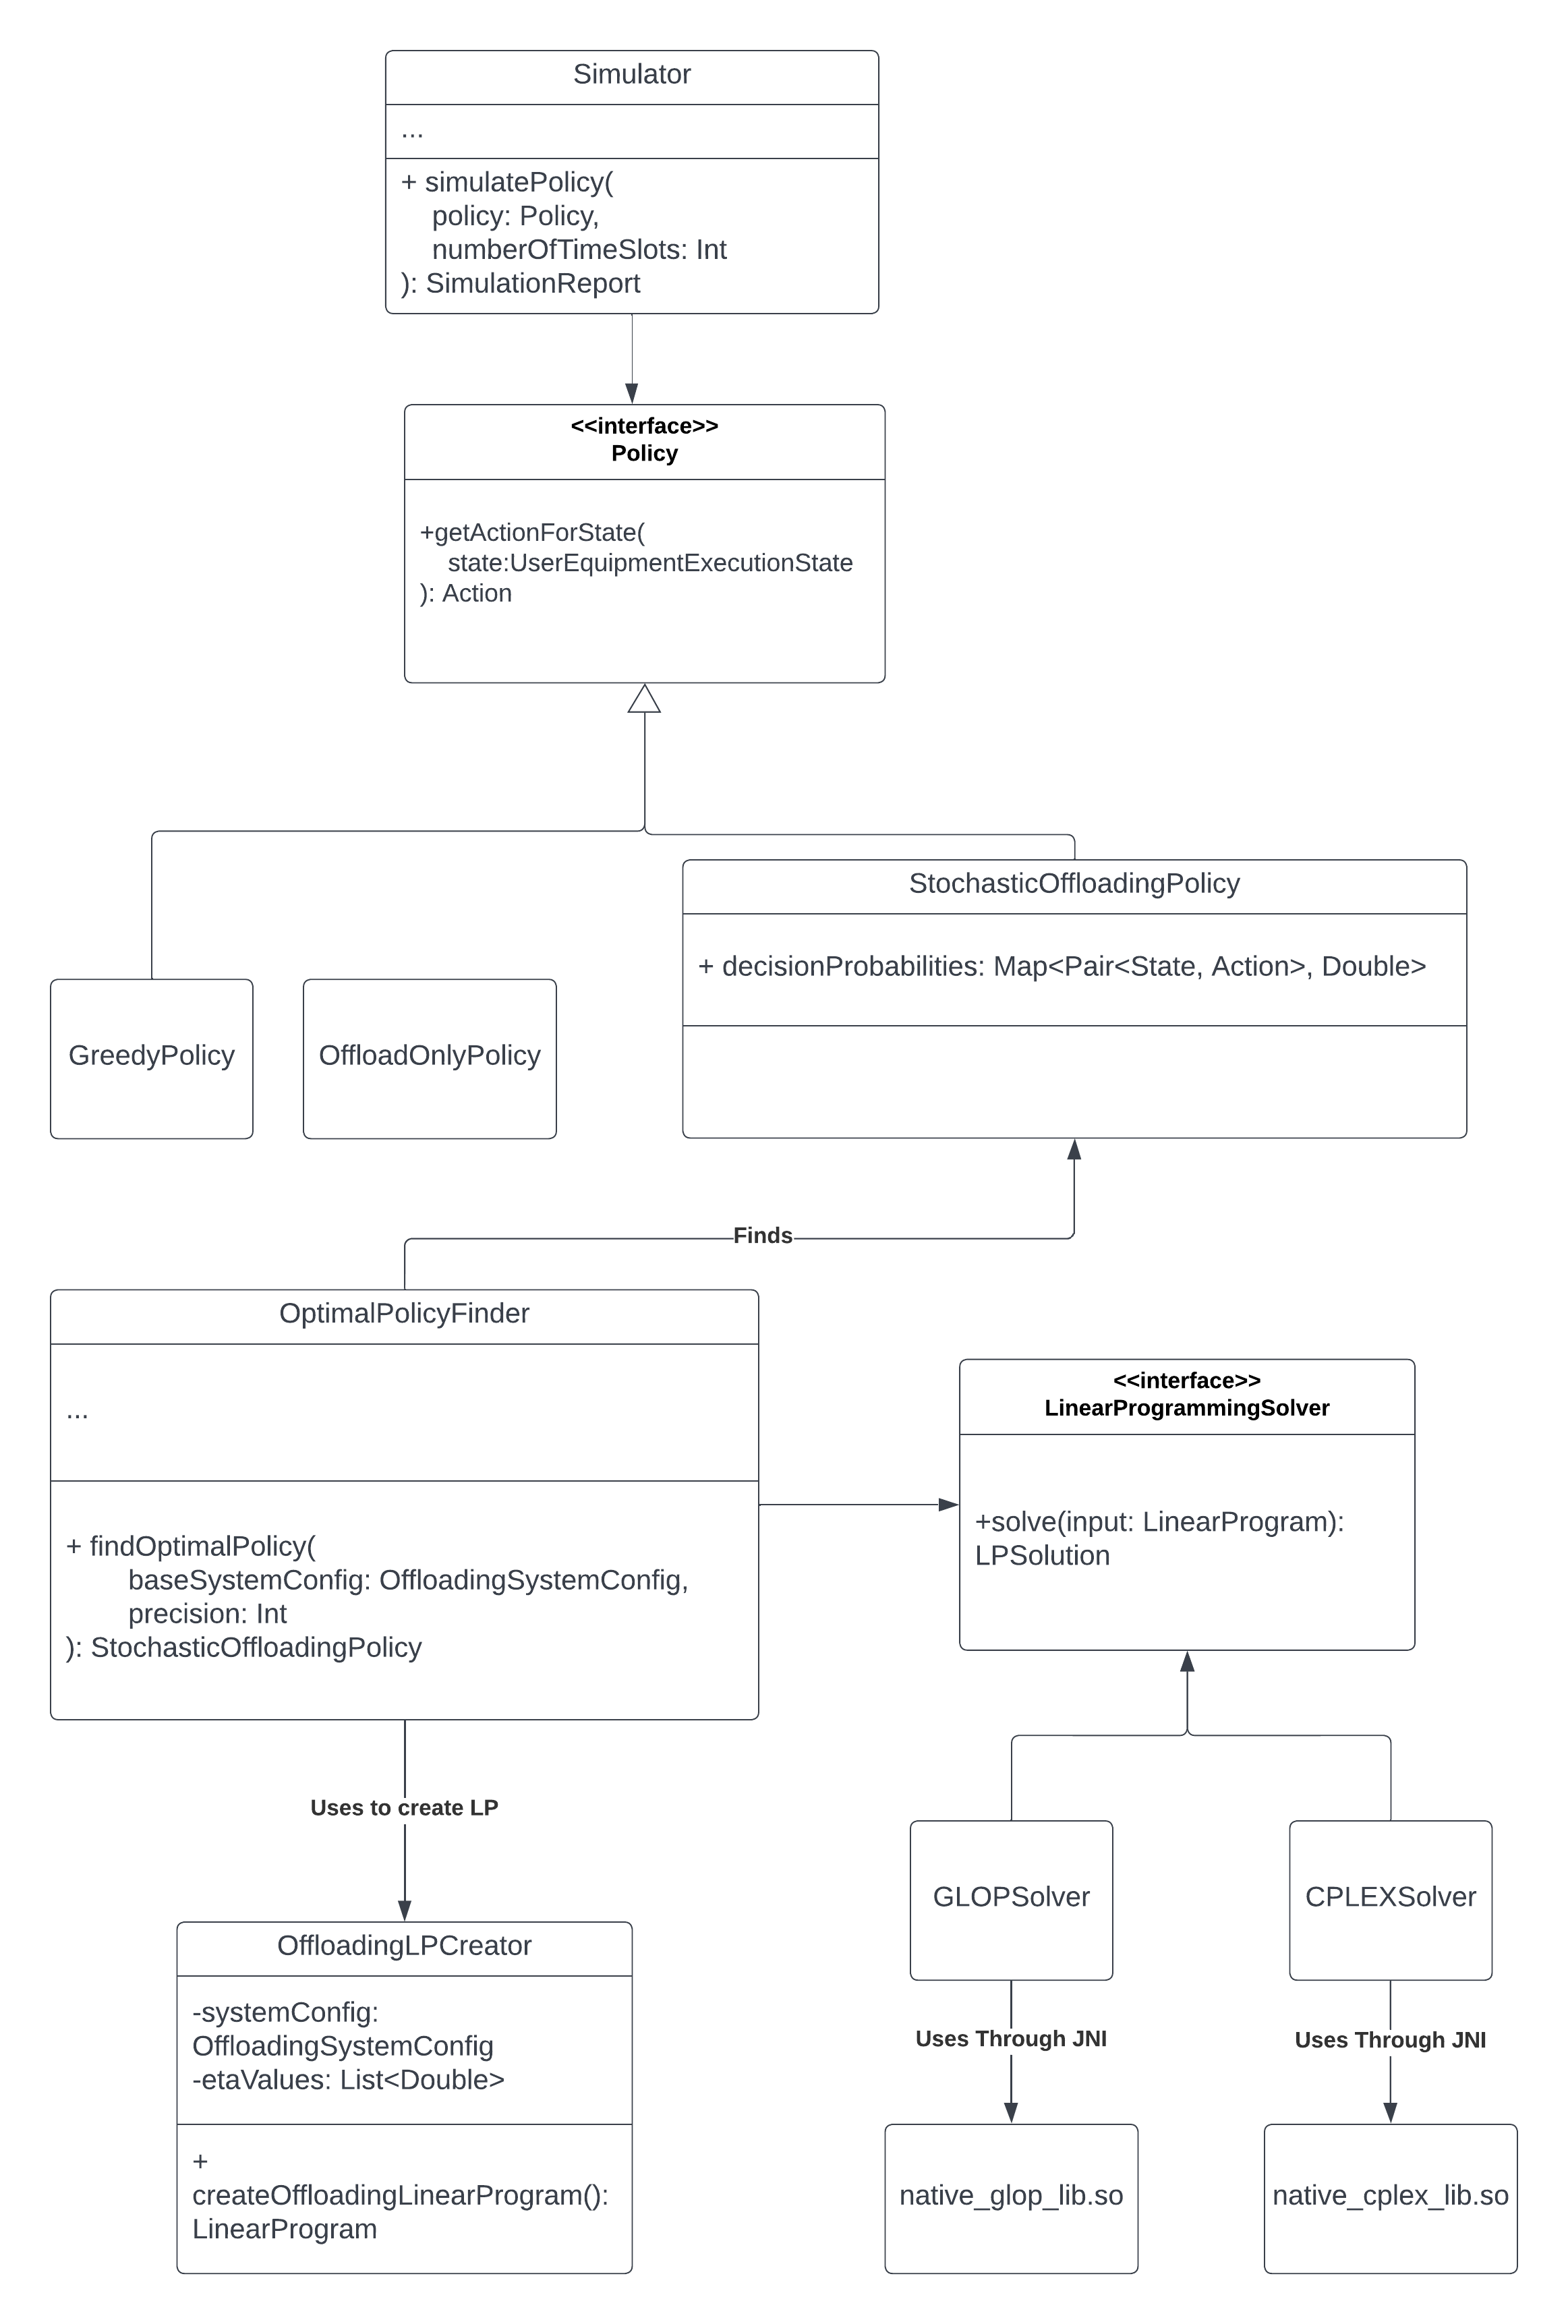
\includegraphics[width=0.9\textwidth]{cdiagram.png}
	\caption{کلاس دیاگرام فریم‌ورک \lr{Kompute}}
\end{figure}
\newpage
\subsection{ساخت و حل یک مسئله تخلیه وظیفه نمونه در \lr{Kompute}}
در کد نمونه زیر مسئله تخلیه وظیفه‌ برای محیط پردازش لبه‌ای با دو صف\footnote{شرایط بر اساس تقسیم‌بندی وظایف به \lr{Heavy} و \lr{Light} در اینترنت اشیا} حل شده است.
\begin{latin}
\begin{lstlisting}[language=Kotlin]
fun main(args: Array<String>) {
	val systemConfig = OffloadingSystemConfig(
		userEquipmentConfig = UserEquipmentConfig(
			stateConfig = UserEquipmentStateConfig(
				taskQueueCapacity = 5,
				tuNumberOfPackets = listOf(1, 3),
				cpuNumberOfSections = listOf(7, 2),
				numberOfQueues = 2
			),
			componentsConfig = UserEquipmentComponentsConfig(
				alpha = listOf(0.4, 0.9),
				beta = 0.90,
				etaConfig = null,
				pTx = 1.0,
				pLocal = 0.8,
				pMax = 1.7
			)
		),
		environmentParameters = EnvironmentParameters(
			nCloud = listOf(1, 1),
			tRx = 0.5,
		)
	)
	
	val optimalPolicy = RangedOptimalPolicyFinder.findOptimalPolicy(
		baseSystemConfig = systemConfig, 
		precision = 10
	)
	/*
	// For multi-threaded execution use this instead:
	
	val optimalPolicy = ConcurrentRangedOptimalPolicyFinder(
		baseSystemConfig = systemConfig
	).findOptimalPolicy(precision = 10, numberOfThreads = 8)
	*/
	
	
	val decisionProbabilities: Map<StateAction, Double>
	= optimalPolicy.stochasticPolicyConfig.decisionProbabilities
	
	println(decisionProbabilities)
}
\end{lstlisting}
\end{latin}
\newpage
\section{نتایج شبیه‌سازی}
در این بخش عملکرد استراتژی یافت شده توسط الگوریتم بخش قبل را با چهار الگوریتم پایه زیر مقایسه می‌کنیم:
\begin{enumerate}
	\item استراتژی فقط تخلیه\LTRfootnote{Offload Only} که همه‌ی وظایف را تخلیه می‌کند
	\item استراتژی حریصانه، تخلیه اول\LTRfootnote{Greedy (Offload First)} که در هر بازه زمانی اگر واحد ارسال یا پردازنده بیکار باشند به هر کدام از آنها یک وظیفه از صفی رندوم تخصیص می‌دهد و در صورتی که تنها یک وظیفه در صف باشد و مجبور به انتخاب بین تخلیه و اجرای محلی باشد، تخلیه را انتخاب می‌کند.
	\item استراتژی حریصانه، محلی اول\LTRfootnote{Greedy (Local First)} که در هر بازه زمانی اگر واحد ارسال یا پردازنده بیکار باشند به هر کدام از آنها یک وظیفه از صفی رندوم تخصیص می‌دهد و در صورتی که تنها یک وظیفه در صف باشد و مجبور به انتخاب بین تخلیه و اجرای محلی باشد، اجرای محلی را انتخاب می‌کند.
	\item استراتژی فقط (اجرای) محلی\LTRfootnote{Local Only}
\end{enumerate}
\newpage
\subsection{شبیه‌سازی تک صف}
با توجه به اینکه روش ارائه شده توسط ما حالت گسترش یافته \cite{Liu} است، ابتدا محیط تست ارائه شده در آن پژوهش را برای تست الگوریتم در نظر می‌گیریم. پارامترهای این محیط در جدول \ref{table:parameters-singlequeue} خلاصه شده اند. نتیجه این آزمایش در شکل \ref{plot:singleQueue} مشاهده می‌شود.

% Please add the following required packages to your document preamble:
\begin{table}[H]
	\centering
	\begin{tabular}{@{}lllllllll@{}}
		\toprule
		\textbf{پارامتر} & $P_1$ & $L_1$ & $\beta$ & $P_{tx}$ & $P_{loc}$ & $P_{max}$ & $C_1$ & $t_{rx}$ \\ \midrule
		مقدار             & 1    & 17   & 0.4  & 1.0 & 0.8  & 1.6  & 1    & 0.0   \\ \bottomrule
	\end{tabular}
	\caption{پارامترهای محیط پردازش لبه‌ای در سناریو تک صف}
	\label{table:parameters-singlequeue}
\end{table}

\begin{figure}[H]
	\centering
	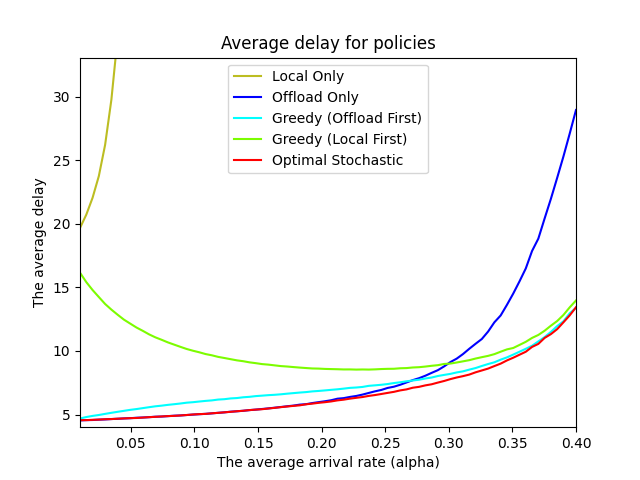
\includegraphics[width=0.7\textwidth]{PlotLiuLimitedSingleQueue.png}
	\caption{تاخیر سرویس به ازای نرخ ورود در حالت تک صف}
	\label{plot:singleQueue}
\end{figure}
همانطور که مشاهده می‌شود استراتژی تخلیه تصادفی یافت شده از تمام الگوریتم‌های پایه بهتر عمل می‌کند و شکل منحنی‌های نمودار با \cite{Liu} مطابقت دارد.
\newpage
\subsubsection{شبیه‌سازی دو صف با یک صف ثابت}
در این قسمت سناریوی تست به این گونه است که به ازای مقادیر مختلف نرخ ورود برای صف شماره یک و مقدار ثابت صف شماره دو مشاهده می‌شود.
\begin{figure}[H]
	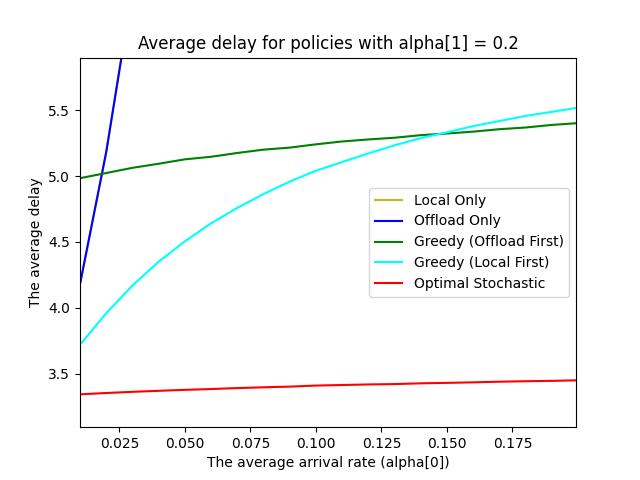
\includegraphics[width=\textwidth]{FixedRanged.png}
\end{figure}
\newpage
\subsubsection{شبیه‌سازی دو صف متغیر}
\begin{figure}[H]
	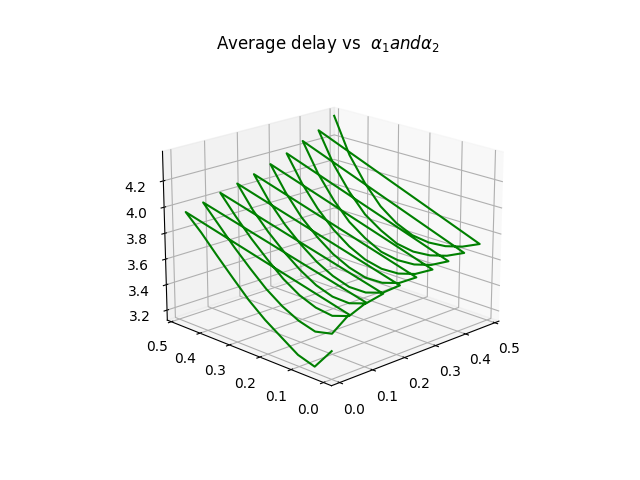
\includegraphics[width=\textwidth]{Plot3d.png}
\end{figure}
\newpage
\subsubsection{تست کارآمدی}
\begin{table}[H]
	\centering
	\begin{latin}		
		\resizebox{\textwidth}{!}{
		\begin{tabular}{llllll}
			\hline
			\textbf{Policy} & Optimal & Local Only & Greedy (Local First) & Greedy (Offload First) & Offload Only \\ \hline
			Value           & 100.0   & 23.33      & 72.49                & 92.95                  & 74.62        \\ \hline
		\end{tabular}
	}
	\end{latin}
\end{table}
\clearpage

\chapter{جمع‌بندی و پیشنهاد‌ها}
در این پژوهش روشی برای بدست آوردن استراتژی تخلیه وظیفه با تاخیر کمینه در شرایط حضور چندین نوع وظیفه در محیط رایانش لبه‌ای معرفی شد. عملکرد این الگوریتم نیز با کمک شبیه‌سازی بررسی شد. در طول انجام این پژوهش ایده‌های مختلفی برای بهبود روش ارائه شده به ذهن ما رسید که برخی از آنها مانند بهینه‌سازی‌های معرفی شده در بخش \ref{sec:optim} پیاده‌سازی شدند. اما برخی از این ایده‌ها به مرحله پیاده‌سازی نرسیدند و پژوهش درباره آنها امکان بهبود روش فعلی را فراهم خواهد کرد. \\

یکی از این موارد کاهش تعداد متغیرهای مسئله برنامه‌ریزی خطی
$\mathcal{P}_2$
(رابطه \ref{eq:p2})
 با استفاده از حذف «تک کنش» ها می‌باشد. پیشتر در بخش \ref{sub:reducevariable} به این موضوع اشاره شد که می‌توان متغیرهایی که متناظر با کنش‌های غیر ممکن هستند را از مسئله بهینه‌سازی 
 $\mathcal{P}_2$
 حذف کرد. با استدلالی مشابه این امکان وجود دارد که متغیرهایی که متناظر با تنها کنش ممکن در یک حالت هستند را از الگوریتم حذف کرد، زیرا مقدار این متغیرها در تعیین استراتژی بهینه نقشی ندارد چون احتمال انتخاب آنها همواره ۱ (قطعی) می‌باشد. با این حال حذف این متغیرها بر خلاف بهینه‌سازی \ref{sub:reducevariable} ساختار زنجیره مارکوف را دگرگون خواهد، بنابراین احتمالا نیازمند تغییر توابع انتقال و/یا تغییر شروط \ref{eq:p2} خواهد شد.
\clearpage
\chapter*{پیوست ۱ - توابع انتقال حالت}

\begin{latin}
	\begin{lstlisting}[language=Kotlin, title=\rl{تابع انتقال حالت به ازای کنش ورودی}]
fun getNextStateRunningAction(
    sourceState: UserEquipmentState,
    action: Action
): UserEquipmentState {	
	return when (action) {
		is Action.NoOperation -> {
			sourceState
		}
		is Action.AddToCPU -> {
			getNextStateAddingToCPU(sourceState, action.queueIndex)
		}
		is Action.AddToTransmissionUnit -> {
			getNextStateAddingToTU(sourceState, action.queueIndex)
		}
		is Action.AddToBothUnits -> {
			getNextStateAddingToBothUnits(
			    sourceState,
			    action.cpuTaskQueueIndex,
			    action.transmissionUnitTaskQueueIndex
			)
		}
	}
}
\end{lstlisting}
\end{latin}
\newpage
\begin{latin}
	\begin{lstlisting}[language=Kotlin, title=\rl{تابع انتقال حالت پایه}]
fun getNextStateAddingToCPU(
    sourceState: UserEquipmentState, 
    queueIndex: Int
): UserEquipmentState {
	require(sourceState.cpuState == 0)
	require(sourceState.taskQueueLengths[queueIndex] > 0)
	
	val updatedLengths = sourceState.taskQueueLengths.decrementedAt(queueIndex)
	
	return sourceState.copy(
	    taskQueueLengths = updatedLengths,
	    cpuState = -1,
	    cpuTaskTypeQueueIndex = queueIndex
	)
}
	\end{lstlisting}
\end{latin}

\begin{latin}
	\begin{lstlisting}[language=Kotlin, title=\rl{تابع انتقال حالت با کنش ارسال توسط واحد ارسال}]
fun getNextStateAddingToTU(
    sourceState: UserEquipmentState,
    queueIndex: Int
): UserEquipmentState {
	require(sourceState.tuState == 0)
	require(sourceState.taskQueueLengths[queueIndex] > 0)
	
	val updatedLengths = sourceState.taskQueueLengths.decrementedAt(queueIndex)

	return sourceState.copy(
	    taskQueueLengths = updateLengths,
	    tuState = 1,
	    tuTaskTypeQueueIndex = queueIndex
	)
}
	\end{lstlisting}
\end{latin}

\newpage
\begin{latin}
	\begin{lstlisting}[language=Kotlin, title=\rl{تابع انتقال حالت با کنش اجرا و ارسال به طور همزمان}]
fun getNextStateAddingToBothUnits(
    sourceState: UserEquipmentState,
    cpuQueueIndex: Int,
    tuTaskQueueIndex: Int
): UserEquipmentState {
	if (cpuQueueIndex == tuTaskQueueIndex) {
		require(sourceState.taskQueueLengths[cpuQueueIndex] > 1)
	} else {
		require(sourceState.taskQueueLengths[cpuQueueIndex] > 0)
		require(sourceState.taskQueueLengths[tuTaskQueueIndex] > 0)
	}
	return getNextStateAddingToCPU(
	    getNextStateAddingToTU(sourceState, tuTaskQueueIndex),
	    cpuQueueIndex
	)
}
	\end{lstlisting}
\end{latin}


\clearpage
\chapter*{پیوست ۲ - تابع ساخت شرط حداکثر توان مصرفی در برنامه خطی}

\begin{latin}
	\begin{lstlisting}[language=Kotlin, title=\rl{تابع ساخت شرط حداکثر توان مصرفی}]
fun getEquation2(): EquationRow {
	val pLoc = systemConfig.pLoc
	val pTx = systemConfig.pTx
	val beta = systemConfig.beta
	val rhsEquation2 = systemConfig.pMax
	val coefficients = mutableListOfZeros(indexMapping.variableCount)
	
	indexMapping.coefficientIndexByStateAction.forEach { (stateAction, index) ->
		val (state, action) = stateAction
		var coefficientValue = 0.0
		
		if (state.isTUActive() 
		|| (action is Action.AddToTransmissionUnit 
		|| action is Action.AddToBothUnits)) {
			coefficientValue += beta * pTx
		}
		
		if (state.isCPUActive() 
		|| (action is Action.AddToCPU) 
		|| (action is Action.AddToBothUnits)) {
			coefficientValue += pLoc
		}
		
		coefficients[index] = coefficientValue
		
	}
	
	return EquationRow(
		coefficients = coefficients,
		rhs = rhsEquation2,
		type = EquationRow.Type.LessThan
	)
}
\end{lstlisting}
\end{latin}
\clearpage
\pagestyle{empty}
{
\onehalfspacing
\bibliographystyle{ieeetr-fa}%{acm-fa}
\bibliography{references/references}
\nocite{*}
}
\pagestyle{fancy}

\onehalfspacing
\chapter*{واژه‌نامه فارسی به انگلیسی}\markboth{واژه‌نامه فارسی به انگلیسی}{واژه‌نامه فارسی به انگلیسی}
\addcontentsline{toc}{chapter}{واژه‌نامه فارسی به انگلیسی}
\thispagestyle{empty}

\englishgloss{Probabilistic}{احتمالی}
\englishgloss{Measure}{اندازه}
\englishgloss{Heuristic}{هیوریستیک}
\englishgloss{Topology}{توپولوژی}
\englishgloss{Cut}{برش}
\englishgloss{Experiment}{آزمایش}
\englishgloss{Social Networks}{شبکه‌های اجتماعی}
\englishgloss{Program Fragment}{قطعه‌برنامه}
\englishgloss{Data Mining}{داده‌کاوی}
\englishgloss{Graph}{گراف}
\englishgloss{Edge}{یال}
\englishgloss{Node}{گره}
\englishgloss{Centrality}{مرکزیت}
\englishgloss{Global}{جهانی}
\englishgloss{Local}{محلی}
\englishgloss{Lovain}{لوون}
\englishgloss{Unstable}{ناپایدار}
\englishgloss{Weblog}{وبلاگ}
\englishgloss{Post}{پست}
\englishgloss{Partition}{افراز}
\englishgloss{Cluster}{خوشه}
\englishgloss{Overlapping}{همپوشان}
\englishgloss{Bridge}{پل}
\englishgloss{Partition}{افراز}
\englishgloss{CLuster}{خوشه}
\chapter*{واژه‌نامه  انگلیسی به  فارسی}\markboth{واژه‌نامه  انگلیسی به  فارسی}{واژه‌نامه  انگلیسی به  فارسی}
\addcontentsline{toc}{chapter}{واژه‌نامه انگلیسی به فارسی}
\thispagestyle{empty}

\persiangloss{مولفه}{Component}
\persiangloss{اجتماع}{Community}
\persiangloss{شبکه‌های پیچیده}{Complex Networks}
\persiangloss{توزیع توانی}{Power-Law Distribution}
\persiangloss{پدیده‌ي دنیای کوچک}{Small-World Phenomenon}
\persiangloss{احتمالی}{Probabilistic}
\persiangloss{تصادفی}{Random}
\persiangloss{محک}{Benchmark}
\persiangloss{نمودار میله‌ای}{Bar-Chart}
\persiangloss{انتخاب دانه}{Seed Selection}
\persiangloss{بسط}{Expansion}
\persiangloss{سیستم اجتماعی}{Social System}
\persiangloss{دنیای واقعی }{Real-World}
\persiangloss{گره دانه}{Seed Node}
\persiangloss{بسط}{Expansion}
\persiangloss{پیرامون}{Boundary}
\persiangloss{کارایی}{Performance}
\persiangloss{گره برشی}{Articulation-Point}
\persiangloss{گره برشی}{Cut-Node}
\persiangloss{یال برشی}{Cut-Edge}
\persiangloss{متخصص}{Expert}
\persiangloss{انسجام}{Cohesiveness}
\persiangloss{جدایی‌پذیری}{Separability}
%\addtocontents{toc}{
    \protect\renewcommand\protect\cftchappresnum{\appendixname~}
    \protect\setlength{\cftchapnumwidth}{\mylenapp}}
   
\chapter{ضمایم}%\label{appendices}
\hypertarget{appendices}{}
\thispagestyle{empty}
\clearpage
\indent{
در این قسمت اطلاعات مربوط به توزیع اندازه‌ی افراز‌های تک تک ۲۲ گراف مورد آزمایش که مربوط به خروجی مرحله‌ی نخست روش
پیشنهادی ماست در دسترس خواننده قرار گرفته است.
}

\begin{figure}[!ht]
  \centering
  \includegraphics[width=0.6\textwidth]{partitions/bio-celegans}
  \caption{توزیع اندازه‌ی افراز‌های گراف
  \lr{celegans}}
\end{figure}

\begin{figure}[!ht]
  \centering
  \includegraphics[width=0.6\textwidth]{partitions/bio-celegans-dir-e}
  \caption{توزیع اندازه‌ی افراز‌های گراف
  \lr{celegans-dir.e}}
\end{figure}

\begin{figure}[!ht]
  \centering
  \includegraphics[width=0.6\textwidth]{partitions/ia-email-univ}
  \caption{توزیع اندازه‌ی افراز‌های گراف
  \lr{email-univ}}
\end{figure}

%%%%%%%%%%%%%%%%%%%%%%%%%%%%%

\begin{figure}[!ht]
  \centering
  \includegraphics[width=0.6\textwidth]{partitions/ia-enron-only}
  \caption{توزیع اندازه‌ی افراز‌های گراف
  \lr{enron-only}}
\end{figure}

\begin{figure}[!ht]
  \centering
  \includegraphics[width=0.6\textwidth]{partitions/ia-fb-messages}
  \caption{توزیع اندازه‌ی افراز‌های گراف
  \lr{fb-messages}}
\end{figure}

\begin{figure}[!ht]
  \centering
  \includegraphics[width=0.6\textwidth]{partitions/ia-infect-hyper}
  \caption{توزیع اندازه‌ی افراز‌های گراف
  \lr{infect-hyper}}
\end{figure}

%%%%%%%%%%%%%%%%%%%%%%%%%%%%%
\clearpage
\begin{figure}[!ht]
  \centering
  \includegraphics[width=0.6\textwidth]{partitions/ia-infect-dublin}
  \caption{توزیع اندازه‌ی افراز‌های گراف
  \lr{infect-dublin}}
\end{figure}

\begin{figure}[!ht]
  \centering
  \includegraphics[width=0.6\textwidth]{partitions/bio-dmela}
  \caption{توزیع اندازه‌ی افراز‌های گراف
  \lr{dmela}}
\end{figure}

\begin{figure}[!ht]
  \centering
  \includegraphics[width=0.6\textwidth]{partitions/bio-diseasome}
  \caption{توزیع اندازه‌ی افراز‌های گراف
  \lr{diseasome}}
\end{figure}

%%%%%%%%%%%%%%%%%%%%%%%%%%%%%
\clearpage
\begin{figure}[!ht]
  \centering
  \includegraphics[width=0.7\textwidth]{partitions/bio-yeast}
  \caption{توزیع اندازه‌ی افراز‌های گراف
  \lr{yeast}}
\end{figure}

\begin{figure}[!ht]
  \centering
  \includegraphics[width=0.7\textwidth]{partitions/ca-netscience}
  \caption{توزیع اندازه‌ی افراز‌های گراف
  \lr{netscience}}
\end{figure}

\begin{figure}[!ht]
  \centering
  \includegraphics[width=0.7\textwidth]{partitions/ca-GrQc}
  \caption{توزیع اندازه‌ی افراز‌های گراف
  \lr{ca-GrQc}}
\end{figure}

%%%%%%%%%%%%%%%%%%%%%%%%%%%%%
\clearpage
\begin{figure}[!ht]
  \centering
  \includegraphics[width=0.99\textwidth]{partitions/ia-wikiTalk}
  \caption{توزیع اندازه‌ی افراز‌های گراف
  \lr{wiki-Talk}}
\end{figure}

\begin{figure}[!ht]
  \centering
  \includegraphics[width=0.99\textwidth]{partitions/ca-AstroPh}
  \caption{توزیع اندازه‌ی افراز‌های گراف
  \lr{AstroPh}}
\end{figure}

\begin{figure}[!ht]
  \centering
  \includegraphics[width=0.99\textwidth]{partitions/soc-douban}
  \caption{توزیع اندازه‌ی افراز‌های گراف
  \lr{douban}}
\end{figure}


\clearpage
\begin{figure}[!ht]
  \centering
  \includegraphics[width=0.99\textwidth]{partitions/ca-CondMat}
  \caption{توزیع اندازه‌ی افراز‌های گراف
  \lr{CondMat}}
\end{figure}

\begin{figure}[!ht]
  \centering
  \includegraphics[width=0.99\textwidth]{partitions/ca-HepPh}
  \caption{توزیع اندازه‌ی افراز‌های گراف
  \lr{HepPh}}
\end{figure}

\begin{figure}[!ht]
  \centering
  \includegraphics[width=0.99\textwidth]{partitions/ia-email-EU}
  \caption{توزیع اندازه‌ی افراز‌های گراف
  \lr{email-EU}}
\end{figure}

%%%%%%%%%%%%%%%%%%%%%%%%%%%%%
\clearpage
\begin{figure}[!ht]
  \centering
  \includegraphics[width=0.99\textwidth]{partitions/inf-power}
  \caption{توزیع اندازه‌ی افراز‌های گراف
  \lr{power}}
\end{figure}

\begin{figure}[!ht]
  \centering
  \includegraphics[width=0.99\textwidth]{partitions/rec-amazon}
  \caption{توزیع اندازه‌ی افراز‌های گراف
  \lr{amazon}}
\end{figure}

\begin{figure}[!ht]
  \centering
  \includegraphics[width=0.99\textwidth]{partitions/ia-reality}
  \caption{توزیع اندازه‌ی افراز‌های گراف
  \lr{reality}}
\end{figure}

%%%%%%%%%%%%%%%%%%%%%%%%%%%%%
\clearpage
\begin{figure}[!ht]
  \centering
  \includegraphics[width=0.99\textwidth]{partitions/ia-enron-large}
  \caption{توزیع اندازه‌ی افراز‌های گراف
  \lr{enron-large}}
\end{figure}

\begin{figure}[!ht]
  \centering
  \includegraphics[width=0.99\textwidth]{partitions/soc-epinions}
  \caption{توزیع اندازه‌ی افراز‌های گراف
  \lr{epinions}}
\end{figure}
\printindex
% !TeX root=main.tex
% در این فایل، عنوان پایان‌نامه، مشخصات خود و چکیده پایان‌نامه را به انگلیسی، وارد کنید.

%%%%%%%%%%%%%%%%%%%%%%%%%%%%%%%%%%%%
\baselineskip=.6cm
\begin{latin}
\latinuniversity{Iran University of Science and Technology}
\latinfaculty{Computer Engineering Department}
\latinsubject{Computer Engineering }
\latinfield{Software Engineering}
\latintitle{A multi-user computation offloading policy to minimize average latency for IoT devices}
\firstlatinsupervisor{Dr. Reza Entezari-Maleki}
%\secondlatinsupervisor{Second Supervisor}
%\firstlatinadvisor{Dr. Einollah Khanjari}
\secondlatinadvisor{Dr. X}
\latinname{\lr{Mohammadmobin}}
\latinsurname{\lr{Dariushhamedani}}
\latinthesisdate{June 2022}
\latinkeywords{Task Offloading, Edge Computing, Markov Chains, Linear Programming, Cloud Computing}
\en-abstract{Edge computing is a distributed computing paradigm that seeks to provide users with lower response times, lower power consumption, and mobility management by bringing computing resources closer to the network edge. Since its introduction, edge computing and its standard implementations, such as Multi-access Edge Computing, have faced one important challenge: How to design efficient task offloading policies? \\ \\ Furthermore, with the rapid growth of the smartphone and IoT industry, many new types of applications have been introduced to the internet, each having different resource needs. Thus, taking into account the heterogeneity of user tasks becomes an essential factor when designing task offloading policies for edge computing environments.\\ \\This paper introduces a method for finding the delay-optimal task offloading policy under the power consumption constraint. The method consists of two steps. First, the offloading system is modeled using Discrete-time Markov Chains. Then, an algorithm based on linear programming is used to find the optimal task offloading policy for the created model. In addition to discussing the problem mathematically, we introduce a new software framework, written in the Kotlin language, which allows users to find the optimal task offloading policy for a given system. This framework can also benchmark the optimal policy's effectiveness using simulation. The current paper is based on \cite{Liu} and uses a similar method to that research.  
}
\latinfirstPage
\end{latin}

\label{LastPage}
\end{document}